%% 
%% Copyright 2007-2020 Elsevier Ltd
%% 
%% This file is part of the 'Elsarticle Bundle'.
%% ---------------------------------------------
%% 
%% It may be distributed under the conditions of the LaTeX Project Public
%% License, either version 1.2 of this license or (at your option) any
%% later version.  The latest version of this license is in
%%    http://www.latex-project.org/lppl.txt
%% and version 1.2 or later is part of all distributions of LaTeX
%% version 1999/12/01 or later.
%% 
%% The list of all files belonging to the 'Elsarticle Bundle' is
%% given in the file `manifest.txt'.
%% 
%% Template article for Elsevier's document class `elsarticle'
%% with harvard style bibliographic references

\documentclass[preprint,12pt,authoryear]{elsarticle}

%% Use the option review to obtain double line spacing
%% \documentclass[authoryear,preprint,review,12pt]{elsarticle}

%% Use the options 1p,twocolumn; 3p; 3p,twocolumn; 5p; or 5p,twocolumn
%% for a journal layout:
%% \documentclass[final,1p,times,authoryear]{elsarticle}
%% \documentclass[final,1p,times,twocolumn,authoryear]{elsarticle}
%% \documentclass[final,3p,times,authoryear]{elsarticle}
%% \documentclass[final,3p,times,twocolumn,authoryear]{elsarticle}
%% \documentclass[final,5p,times,authoryear]{elsarticle}
%% \documentclass[final,5p,times,twocolumn,authoryear]{elsarticle}

%% For including figures, graphicx.sty has been loaded in
%% elsarticle.cls. If you prefer to use the old commands
%% please give \usepackage{epsfig}

%% The amssymb package provides various useful mathematical symbols
\usepackage{amsmath,amssymb}
%% The amsthm package provides extended theorem environments
\usepackage{amsthm}
\usepackage{lipsum}

\newcommand*{\FilePath}{C:/Users/agbenso/Desktop/BESS_Cost_Analysis/Manuscript}

\usepackage{graphicx}
\graphicspath{ {./graphs/} } 
\usepackage{subfig}
\usepackage{multirow}
\usepackage{tabularx}
\usepackage{longtable}

\makeatletter
\def\@cline#1-#2\@nil{%
  \omit
  \@multicnt#1%
  \advance\@multispan\m@ne
  \ifnum\@multicnt=\@ne\@firstofone{&\omit}\fi
  \@multicnt#2%
  \advance\@multicnt-#1%
  \advance\@multispan\@ne
  \leaders\hrule\@height\arrayrulewidth\hfill
  \cr
  \noalign{\nobreak\vskip-\arrayrulewidth}}
\makeatother

\usepackage{afterpage}
\usepackage{url}
\usepackage{pdflscape}
\usepackage{hyperref}
\usepackage{pifont}
\usepackage{bbold}

\defcitealias{EPRI2020}{EPRI (2020)}
\defcitealias{PCEPI}{BEA, 2022}
\defcitealias{BEA_county_income}{BEA, 2021}
\defcitealias{BLS_OEWS}{BLS, 2022}
\defcitealias{CPUC_IRP}{CPUC, 2019}
\defcitealias{D16_06_055}{CPUC, 2016}
\defcitealias{D20_01_021}{CPUC, 2020}
\defcitealias{SGIP_2022}{SGIP, 2022}
\defcitealias{ATB2022}{NREL, 2022}

% define large "struts", as suggested by Claudio Beccari in a piece in TeX and TUG News, Vol. 2, 1993.
\newcommand\Tstrut{\rule{0pt}{2.6ex}}         % = `top' strut
\newcommand\Bstrut{\rule[-1.6ex]{0pt}{0pt}}   % = `bottom' strut

% define small "struts", as suggested by Claudio Beccari in a piece in TeX and TUG News, Vol. 2, 1993.
\newcommand\tstrut{\rule{0pt}{2.5ex}}         % = `top' strut
\newcommand\bstrut{\rule[-1.0ex]{0pt}{0pt}}   % = `bottom' strut

\newcommand\Xst{\textsuperscript{st}}
\newcommand\Xnd{\textsuperscript{nd}}
\newcommand\Xrd{\textsuperscript{rd}}
\newcommand\Xth{\textsuperscript{th}}

%% The lineno packages adds line numbers. Start line numbering with
%% \begin{linenumbers}, end it with \end{linenumbers}. Or switch it on
%% for the whole article with \linenumbers.
%% \usepackage{lineno}

\journal{Energy Reports}

\begin{document}

\begin{frontmatter}

%% Title, authors and addresses

%% use the tnoteref command within \title for footnotes;
%% use the tnotetext command for theassociated footnote;
%% use the fnref command within \author or \affiliation for footnotes;
%% use the fntext command for theassociated footnote;
%% use the corref command within \author for corresponding author footnotes;
%% use the cortext command for theassociated footnote;
%% use the ead command for the email address,
%% and the form \ead[url] for the home page:
%% \title{Title\tnoteref{label1}}
%% \tnotetext[label1]{}
%% \author{Name\corref{cor1}\fnref{label2}}
%% \ead{email address}
%% \ead[url]{home page}
%% \fntext[label2]{}
%% \cortext[cor1]{}
%% \affiliation{organization={},
%%            addressline={}, 
%%            city={},
%%            postcode={}, 
%%            state={},
%%            country={}
%% \fntext[label3]{}

\title{Customized Predictions of the Installed Cost of Behind-the-Meter Battery Energy Storage Systems}

%% use optional labels to link authors explicitly to addresses:
%% \author[label1,label2]{}
%% \affiliation[label1]{organization={},
%%             addressline={},
%%             city={},
%%             postcode={},
%%             state={},
%%             country={}}
%%
%% \affiliation[label2]{organization={},
%%             addressline={},
%%             city={},
%%             postcode={},
%%             state={},
%%             country={}}

\author[agb]{Andrew G. Benson}

\ead{agbenson1991@gmail.com}
\ead[url]{https://github.com/a-g-benson}

\affiliation[agb]{organization={Sandia National Laboratories$^1$},
            addressline={P.O. Box 5800}, 
            city={Albuquerque},
            state={NM},
            postcode={87185-1108},
            country={USA}}

\fntext[SNL_contract_language]{Sandia National Laboratories is a multi-mission laboratory managed and operated by National Technology and Engineering Solutions of Sandia, LLC., a wholly owned subsidiary of Honeywell International, Inc., for the U.S. Department of Energy National Nuclear Security Administration under contract DE-NA-0003525. This paper describes objective technical results and analysis derived from research conducted at the time of the author's employment at Sandia National Laboratories. Any subjective views or opinions that might be expressed in the paper do not necessarily represent the views of the U.S. Department of Energy or the United States Government. The author would like to thank Dr. Imre Gyuk, Director of Energy Storage Research, Office of Electricity Delivery and Energy Reliability for his support of this research.}

\begin{abstract}

Behind-the-meter (BTM) battery energy storage systems (BESS) are undergoing rapid deployment. Simple equations to estimate the installed cost of BTM BESS are often necessary when a rigorous, bottom-up cost estimate is not available or not appropriate, in applications such as energy system modeling, informing a BESS sizing decision, and cost benchmarking. Drawing on project-level data from California, I estimate several predictive regression models of the installed cost of a BTM BESS as a function of energy capacity and power capacity. The models are evaluated for in-sample goodness-of-fit and out-of-sample predictive accuracy. The results of these analyses indicate stronger empirical support for models with natural log transformations of installed cost, energy, and power as compared against widely-used models that posit a linear relationship among the untransformed versions of these variables. Building on these results, I present a logarithmic model that can predict installed cost conditional on energy capacity, power capacity, AC or DC coupling with distributed generation, customer sector, and local wages for electricians. I document how the model can be easily extrapolated to future years, either with forecasts from other sources or by re-estimating the parameters with the latest data.

\end{abstract}

%%Graphical abstract
%%\begin{graphicalabstract}
%\includegraphics{grabs}
%%\end{graphicalabstract}

%%Research highlights
%%\begin{highlights}
%%\item Research highlight 1
%%\item Research highlight 2
%%\end{highlights}

\begin{keyword}
%% keywords here, in the form: keyword \sep keyword

%% PACS codes here, in the form: \PACS code \sep code

%% MSC codes here, in the form: \MSC code \sep code
%% or \MSC[2008] code \sep code (2000 is the default)

energy storage \sep batteries \sep behind-the-meter \sep cost \sep model selection \sep prediction

\end{keyword}

\end{frontmatter}

%% \linenumbers

%% main text
\section{Introduction}\label{sec:intro}

Behind-the-meter (BTM) battery energy storage systems (BESS) are undergoing the early stages of rapid, widespread deployment. An accurate understanding of their costs and benefits is relevant to analysis and decision-making in a variety of contexts, ranging from a costumer's purchase decision to energy system modeling. In many contexts, it is not feasible or appropriate to develop a highly-detailed, bottom-up cost estimate of a BESS at a specific site meeting a customer's particular requirements and a choice of equipment. For example, in a cost benchmarking study, a researcher would compare transacted or quoted prices against a synthetic cost benchmark, which must abstract from site-specifc conditions and customer-specific requirements. To address this need, I develop a predictive regression model of the installed cost---the sum of all upfront costs, including the battery module, installation labor, permitting, and project overhead---of BTM BESS. The model takes as inputs usable energy capacity (kWh), power capacity (kW), type of coupling with distributed generation (AC, DC, or none), local median wage for electricians, host customer sector (residential or non-residential), and year of installation. 

In Section \ref{sec:lit_review}, I review the prior literature that estimates or forecasts the installed cost of BTM BESS. Typically, prior works have estimated the installed cost of a representative system or an average specific cost (\$ per kWh). A handful of studies provide an equation that can generate a prediction for user-determined values of energy capacity and power capacity. All such equations have been linear in functional form and their parameters have been derived from expert elicitation, literature review, or bottom-up engineering estimates. In this work, I show that the linear assumption of prior work is not empirically supported by a large-N, project-level dataset of BTM BESS from California, introduced in Section \ref{sec:data}. Instead, models with natural log transformations of installed cost, energy capacity, and power capacity exhibit the best fit to the data. The model selection process is summarized in Section \ref{sec:model_selection} and justified in detail in \ref{apdx:methodology}.

The results of the model comparison favor a translog specification \citep{kmenta1967}, followed closely by Cobb-Douglas \citep{cobbdouglas1928}. The improvement in goodness-of-fit of a translog model compared against Cobb-Douglas is trivial in magnitude; in most respects, the differences between the results of the two models are negligible. For example, both models find economies of scale of about a 29\% reduction in cost per kWh for a 10-fold increase in system size. Both models exhibit time trends in the residential sector consistent with a price war in 2017 followed by a gradual recovery in (inflation-adjusted) prices until converging with the cost level of the non-residential sector in 2021. Given these similarities, I present and discuss the results of the translog model in Section \ref{sec:results} and reserve the same for the Cobb-Douglas model to \ref{apdx:cobb_douglas}.

However, the translog and Cobb-Douglas models generate substantially different predictions for BTM BESS with discharge durations outside the range of the most common values---1.7 to 2.64 hours---that are present in the data. The choice of functional form determines the marginal cost of energy capacity: while Cobb-Douglas predicts declining marginal costs, translog predicts increasing marginal costs that are \textit{a priori} not credible. Nevertheless, I find that the translog model exhibits better fit to the data for BTM BESS with uncommon discharge durations; the Cobb-Douglas estimates of marginal cost of energy capacity are not robust to alternative evaluations of model fit. Real-world data on BTM BESS with more dispersion in discharge duration will be necessary to validate, refine, or overturn these results. When such data become available, the same model selection process presented herein can be applied to determine the most suitable model.

 In Section \ref{sec:prediction}, I present a simple method of updating the relevant parameter to extrapolate the translog or Cobb-Douglas model to future years or jurisdictions outside of California. Next, I investigate the distribution of residuals and generate empirically-derived prediction intervals. Finally, I conduct an exercise to validate and compare the forecast accuracy of the translog, Cobb-Douglas, and linear models of the installed cost BTM BESS. The forecast validation exercise relies strictly on data from 2013 to 2021 to predict values of installed cost for BTM BESS interconnected in 2022. The exercise finds greater forecast accuracy for an empirically-estimated translog model than a leading forecast that relies on a linear model of cost and bottom-up, techno-economic analysis to calibrate its parameters.
 
 In Section \ref{sec:conclusion}, I conclude and consider directions for future research. Section \ref{sec:data_avail} provides a link to the online data appendix and replication code.

\section{Literature Review}\label{sec:lit_review}

Prior literature has estimated historical, current, and future costs of battery energy storage systems. Typical studies and industry reports focus on the estimation of a measure of central tendency, usually expressed as the average cost per kilowatt-hour of energy capacity. Table \ref{tab:cost_est_BTM} presents a summary of recent estimates for BTM BESS. In light of varied dates of installation, system sizes, and system configurations, the different estimates reflect differing asumptions as much as they reflect differing cost judgements. The median values (estimated separately for residential and non-residential sectors) of the collected estimates is reported for the sake of an approximate summary. The large cost discrepancy between residential (\$1,183 per kWh) and non-residential systems (\$375 per kWh) reflects economies of scale.

A single figure of merit for installed cost is suitable for many purposes but inadequate for others. Among its limitations, a single metric cannot credibly inform industry participants and energy system modelers of the costs of varying system size parameters. Economies of scale are an important consideration, as well as the marginal cost of energy and power capacity. As interest in long-duration energy storage grows, it will be important to model how the cost of BTM BESS varies with discharge duration. A further limitation of a single cost metric is the absence of information about statistical dispersion, without which statistical inference is impossible. Below, I discuss studies that do address these limitations and remark on how the present work improves upon prior methodology.

\subsection{Linear Models of Cost}\label{sec:linear_lit}

Several prior studies---both of front-of-the-meter (FTM) and BTM BESS---have sought to generalize beyond the total cost of a representative system or a single estimate of cost per kWh. \citet{dietrich2018}, \citet{schmidt2019}, \citet{comello2019}, and \citet{augustineblair2021} employ an equation that governs how installed cost ($C_i$) scales with energy capacity ($E_i$) and power capacity ($P_i$). All of these works assume a linear function of the following form:

\begin{equation}\label{eq:linear_model}
    C_i = \alpha + \beta_{1} E_i + \beta_{2} P_i + \varepsilon_i
\end{equation}

In studies that forecast future costs, the parameters $\alpha$, $\beta_1$, and $\beta_2$ are allowed to vary (generally, decline) over time. Some studies \citep{schmidt2019,comello2019} omit the fixed cost term $\alpha$, as does the California Public Utilities Commission (CPUC) in its integrated resource planning \citepalias[][pp. 58-60]{CPUC_IRP}. 

Eq. \ref{eq:linear_model} is generally justified on the grounds that the installed cost of a BESS can be decomposed into fixed costs ($\alpha$), costs that scale with the number of batteries ($\beta_1 E_i$), and costs that scale with the size of the power conversion system ($\beta_2 P_i$). Such a model is intuitively appealing, which likely explains its widespread use. However, it implies strong assumptions. Under a linear model, economies of scale only arise insofar as larger systems can spread the fixed cost over a larger number of kilowatts and/or kilowatt-hours. The marginal costs of energy capacity and power capacity are constant. The work of \citet{tsai2020} contains a rare example of non-linearity in the specific costs of energy and power capacity, as presented in Table \ref{tab:tsai_2021}. The authors report that these figures are sourced from an undisclosed system integrator based in Taiwan.

\begin{table}[h!]
\centering
	\subfloat[\centering Energy Capacity Costs]{{\begin{tabular}{|ccc|}
\hline
\begin{tabular}[c]{@{}c@{}}Number of\\ Battery\\ Racks\end{tabular} & \begin{tabular}[c]{@{}c@{}}Size of\\ Shipping\\ Container\end{tabular} & \$/kWh \\ \hline
1 - 2 & 10 ft & \$340 \\
3 - 6 & 20 ft & \$290 \\
7 - 10 & 40 ft & \$280 \\ \hline
\end{tabular}}}
	\subfloat[\centering Power Capacity Costs]{{\begin{tabular}{|cc|}
\hline
\begin{tabular}[c]{@{}c@{}}Power\\ Capacity\end{tabular} & \$/kW \\ \hline
100 kW & \$186 \\
250 kW & \$123 \\
500 kW & \$100 \\
700 kW & \$82 \\ \hline
\end{tabular}}}
\caption{Specific Costs from \citet[][p. 203,739]{tsai2020}}\label{tab:tsai_2021}
\end{table}

As I show in \ref{apdx:time_var_coef}, a linear model fits real-world data rather poorly. Most of the aforementioned studies parameterize Eq. \ref{eq:linear_model} by means of meta-analysis or expert elicitation. The exception is \citet{dietrich2018}, who estimate a linear model of module costs for BTM BESS by ordinary least squares (OLS) using a sample of 79 battery models. Lacking data on installation costs, they assume a representative value and add it to the estimate of $\alpha$.  Although \citet{dietrich2018} estimate non-linear models of the costs of PV solar arrays and inverters, they assume a linear functional form for BTM BESS and do not evaluate alternative functional forms. I contribute to the literature through an explicit and documented methodology for model selection. The models that exhibit the best fit to the data I rely on this work---namely, Cobb-Douglas and translog---have a long history \citep{cobbdouglas1928, kmenta1967} and have been applied in a variety of industries, ranging from life insurance \citep{segal2003}, to nuclear power \citep{berthelemy2015}, to agriculture \citep{ray1982}, to railroads \citep{bogart2010}.

\subsection{Treatment of Uncertainty}\label{sec:lit_uncertainty}

In works forecasting future costs of BTM BESS, the forecasts are often presented with a range of possible values, representing uncertainty in the chosen measure of central tendency. For example, \citet{augustineblair2021} present a ``moderate" forecast (best estimate), a ``conservative" forecast (upper bound), and an ``advanced" forecast (lower bound), which inform assumptions in the correspondingly named scenarios of the Annual Technology Baseline (ATB) of the U.S. National Renewable Technology Laboratory \citepalias{ATB2022}. While such an uncertainty range can have many applications (e.g. sensitivity analysis of scenarios for future energy systems), it is not appropriate for the purposes of generating a prediction interval around the best estimate of the cost of an individual BESS.\footnote{Throughout this work, I use ``prediction interval'' to strictly refer to this sort of uncertainty range. I reserve ``confidence interval'' for uncertainty ranges around the estimate of the conditional mean or a particular parameter.} As I show in Subsection \ref{sec:validation}, the interval bounded by the conservative and advanced ATB forecasts of installed cost only contains 5.7\% of the observations for 2022. Any particular project can face site-specific conditions or design requirements with idiosyncratic effects on costs, particularly behind-the-meter where it must interface with a customer's existing electrical system. These two sources of uncertainty---uncertainty in the future mean vs. variability in individual outcomes---are distinct issues.

In studies that do address the variability in individual outcomes \citep{battke2013,zakeri2015,obi2017,schmidt2019}, the distributional assumptions that underlie the uncertainties their calculations have a limited empirical basis in project-level variance. These works rely on a mixture of expert elicitation and meta-analysis of prior literature, and then make distributional assumptions based on the dispersion in those estimates. For example, \citet{schmidt2019} report ``the Monte Carlo analysis simulates 500 levelized cost of storage calculations per technology and application based on random values from an 80\% confidence interval of the attributed normal distribution of the parameter, corresponding to 1.285 standard deviations from the mean.'' \citet{battke2013} write that ``A PERT distribution was assumed for the stochastic input parameters because this distribution is explicitly recommended to be used to model expert estimates as it is less sensitive to extreme values, for instance in comparison to the triangular distribution.'' 

In contrast to these prior works, the present work generates prediction intervals from large-N, project-level data. In Subsection \ref{sec:prediction_interval}, I examine the empirical distribution of the residuals---the discrepancy between the predicted and the observed value of installed cost---to formulate prediction intervals. I show that, for my preferred model specifications, the distribution of residuals is closely approximated by a Laplace distribution. I calibrate the parameters of a Laplace distribution to match the empirical distribution and use it compute the bounds of a 95\% prediction interval. In Subsection \ref{sec:validation}, I show that the resulting prediction intervals are well-calibrated: 93.6\% of year 2022 observations fall within their associated 95\% prediction interval.

\subsection{Theoretical Foundations of Statistical Model Selection}

As previously mentioned, a statistical approach to model selection has not been implemented in prior literature on the installed cost of BTM BESS. A statistical approach is necessary to rigorously assess whether to and what extent theoretical models used in research conform to empirical observation. I adopt the Akaike Information Criterion (AIC) \citep{akaike1974} as the primary model selection criterion of this work. The AIC has been described as ``a simple, effective, and very general methodology for selecting a parsimonious model for the analysis of empirical data'' \citep[p. 32]{burnhamanderson1998} and is widely used.\footnote{\cite{akaike1974} has over 60,000 citations on Google Scholar as of the time of writing.} While some researchers prefer the Bayesian Information Criterion (BIC) \citep{burnham2004}, in my setting the model selection decision is not sensitive to the selection criterion.

\begin{landscape}
\begin{table}[h]
\begin{tabular}{rccccclc}
\hline
\multicolumn{1}{c}{\multirow{2}{*}{Citation \Tstrut }} & \multirow{2}{*}{\Tstrut \begin{tabular}[c]{@{}c@{}}Date of \\ Installation\end{tabular}} & \multirow{2}{*}{\begin{tabular}[c]{@{}c@{}}Customer\\ Sector\end{tabular}} & \multicolumn{2}{c}{\Tstrut  Scale}                           & \multirow{2}{*}{\$/kWh} & \multicolumn{1}{c}{\multirow{2}{*}{\begin{tabular}[c]{@{}c@{}}System\\ Configuration\end{tabular}}} & \multirow{2}{*}{Notes} \\ \cline{4-5}
                          &                                                                                 &                                                                            & kW \Tstrut                      & KWh                      &                         & \multicolumn{1}{c}{}                                                                                &                        \\ \hline
\citet{augustineblair2021}  & 2019                                                                         & Residential                                                                & 5                        & 12.5                      & \$1,570                 & standalone                                                                                          &    ---                    \\
\citet{augustineblair2021}  & 2019                                                                         & Residential                                                                & 5                        & 12.5                      & \$1,041                 & \multicolumn{2}{l}{paired with 3.5 to 15 kW PV \,\,  ---}                                                          \\
\citet{ramasamy2021}  & 2021 Q1                                                                         & Residential                                                                & 5                        & 7.5                      & \$1,904                 & standalone                                                                                          &     ---                   \\
\citet{ramasamy2021}   & 2021 Q1                                                                         & Residential                                                                & 5                        & 12.5                     & \$1,337                 & standalone                                                                                          &         ---               \\
\citet{ramasamy2021}   & 2021 Q1                                                                         & Residential                                                                & 5                        & 12.5                     & \$920                   & paired with 7.15 kW PV                                                                              &   DC-coupled                    \\
\citet{ramasamy2021}   & 2021 Q1                                                                         & Residential                                                                & 10                       & 25                       & \$1,068                 & standalone                                                                                          &          ---             \\
\citet{LazardLCOSv7}            & 2021                                                                            & Residential                                                                & 5                        & 25                       & \$817                   & paired with 10 kW PV                                                                                & high case              \\
\citet{LazardLCOSv7}                & 2021                                                                            & Residential                                                                & 5                        & 25                       & \$477                   & paired with 10 kW PV                                                                                & low case               \\ 
\citet{EnergySage2021}                & 2020 Q3                                                                            & Residential                                                                & ---           & ~10                       & \$1,128                   & paired with PV                                                                                &        ---        \\
\citet{EnergySage2021}                & 2020 Q4                                                                            & Residential                                                                & ---           & ~10                       & \$1,183                   & paired with PV                                                                                &     ---          \\
\citet{EnergySage2021}                & 2021 Q1                                                                            & Residential                                                                & ---           & ~10                       & \$1,183                   & paired with PV                                                                                &     ---         \\
\citet{EnergySage2021}                & 2021 Q2                                                                            & Residential                                                                & ---          & ~10                       & \$1,241                   & paired with PV                                                                                &      ---        \\
\citet{EnergySage2022a}                & 2021 Q3                                                                            & Residential                                                                & ---           & ~10                       & \$1,344                   & paired with PV                                                                                &     ---         \\
\citet{EnergySage2022a}                & 2021 Q4                                                                            & Residential                                                                & ---           & ~10                       & \$1,289                   & paired with PV                                                                                &     ---         \\
\citet{EnergySage2022b}                & 2021 Q1/2                                                                            & Residential                                                                & ---          & ~10                       & \$1,290                   & paired with PV                                                                                &      ---        \\ \hline
\multicolumn{1}{c}{Median}                     &                                                                                 & Residential                                                                &                          &                          & \$1,183                   &                                                                                                     &                        \\ \hline
\citet{augustineblair2021}  & 2019                                                                         & Non-Residential                                                               & 600                       & 2400                     & \$485               & standalone                                                                                          &               ---         \\
\citet{augustineblair2021}  & 2019                                                                         & Non-Residential                                                               & 600                       & 2400                    & \$308                & paired with 1 MW PV                                                                                          &        ---                \\
\citet{ramasamy2021}   & 2021 Q1                                                                         & Non-Residential                                                                 & 600                      & 2400                     & \$481                   & standalone                                                                                          &          ---              \\
\citet{ramasamy2021}   & 2021 Q1                                                                         & Non-Residential                                                                 & 600                      & 2400                     & \$375                   & paired with 1 MW PV                                                                                 &        DC-coupled               \\
\citet{LazardLCOSv7}               & 2021                                                                            & Non-Residential                                                            & 1000 & 2000 & \$375                   & standalone                                                                                          & high case              \\
\citet{LazardLCOSv7}                & 2021                                                                            & Non-Residential                                                              & 1000 & 2000 & \$314                   & standalone                                                                                          & low case               \\
\citet{LazardLCOSv7}                & 2021                                                                            & Non-Residential                                                             & 1000 & 2000 & \$713                   & paired with 1 MW PV                                                                                 & high case              \\
\citet{LazardLCOSv7}               & 2021                                                                            & Non-Residential                                                         & 1000 & 2000 & \$328                   & paired with 1 MW PV                                                                                 & low case               \\
\citet{viswanathan2022}    & 2021                                                                            & Non-Residential                                                              & 1000                     & 4000                     & \$448                   & standalone                                                                                          &                 ---       \\ \hline
\multicolumn{1}{c}{Median}                     &                                                           & Non-Residential                                              &     &      & \$375                   &                                                                                                     &                       \\\hline
\end{tabular}
\caption{Recent estimates of the cost of BTM Li-ion BESS.}\label{tab:cost_est_BTM}
\end{table}
\end{landscape}


\section{Data}\label{sec:data}

\subsection{California's Self-Generation Incentive Program}\label{sec:data_SGIP}

The Self-Generation Incentive Program (SGIP) provides subsidies for the installation of distributed energy resources to customers of California's largest investor-owned utilities (IOUs), including those in the service territory of electric publicly-owned utilities (POUs) but natural gas IOUs.\footnote{Examples of such customers include residents of the City of Los Angeles (LADWP/SoCalGas) and Sacramento County (SMUD/PG\&E)}. The California Public Utilities Commission (CPUC) sets the rules governing the program, such as eligiblity and reimbursement rate; the IOUs administer the program\footnote{Except in the case of San Diego Gas \& Electric, in whose service territory a non-profit organization has been tasked with program administration.} When it was originally established in 2001 in response to the California electricity crisis, SGIP exclusively provided incentives for distributed generation and waste heat recovery. Since that time, the governing legislation and CPUC rules have evolved, most notably in 2016 when the CPUC allocated 75\% of the SGIP budget to energy storage \citepalias{D16_06_055}. For the period 2020-2024, 88\% of the SGIP budget is allocated to energy storage \citepalias{D20_01_021}.

Initially, SGIP provided subsidies to BTM BESS on a per watt basis, i.e., proportionate to the AC power capacity of the system. The amount was revised gradually downwards, from \$2/W in 2011 to \$1.31/W in 2016. In 2017, the rules were radically overhauled. The subsidy for BTM BESS is now proportionate to the energy capacity of the system (in watt-hours), adjusted for depth-of-discharge, ancillary loads, and inverter losses. SGIP subsidy rates also vary according to the discharge duration--i.e. the number of hours over which the BESS can discharge at its maximum rated power capacity, starting from a full state of charge. SGIP penalizes applicants with longer discharge durations by awarding only a percentage of the incentive to which the applicant would otherwise be entitled, as presented in Table \ref{tab:LD_penalties}. In 2020, the penalty for longer durations was lessened, although systems with discharge durations in excess of 6 hours remain ineligible for SGIP.

%Furthermore, the rate of the subsidy is structured to ``step down'' after a specified amount of program funds are exhausted for various classes of customers. Five ``incentive steps'' were originally established, later supplemented to seven for residential customers, with amounts ranging from \$0.50/Wh in Step 1 to \$0.25/Wh in Step 5 and \$0.15/Wh in Step 7. The generosity of the subsidy is monotonically decreasing in the number of the ``step.''

%The step-down in subsidy rate occurs independently by program administrator and ``budget category.'' Budget categories consist of classes of customers defined by the program rules, of which there are presently seven. The first two budget categories are open to any and all residential and non-residential customers of the IOUs. Three ``equity'' budget categories are reserved for: low-income residential customers; state, local, and tribal governments; non-profits; educational institutions; and small businesses. A final two categories are for residential and non-residential customers in the San Joaquin Valley. Customers qualifying for these special budget categories are eligible for exceptionally generous incentives, as high as \$1.00/Wh.

%For non-residential SGIP participants claiming the federal Investment Tax Credit for their BESS (which must paired with a solar PV installation under federal tax law), the SGIP subsidy is reduced by 28\%. 

\begin{table}[t]
\centering
\begin{tabular}{|c|c|c|}\hline
Discharge & 2017 to & 2020 to  \\
Duration & 2019 & Present  \\ \hline
$0 <$ hours $\leq 2$   &   100\%   &   100\%    \\
$2 <$ hours $\leq 4$    &   50\%   &    100\%   \\
$4 <$ hours $\leq 6$      &   25\%   &   50\%   \\
\multicolumn{1}{|l|}{$6 <$ hours}  &    0\%  &    0\%    \\\hline
\end{tabular}
\caption{SGIP Generosity as a Percentage of the Baseline Incentive, by Discharge Duration and Program Year.}\label{tab:LD_penalties}
\end{table}

SGIP administrative data are publicly available from a website maintained by the program administrators.\footnote{\url{https://www.selfgenca.com/report/public/}} The dataset encompasses every application for SGIP funds, dating back to the program's inception, and is updated daily. For the purposes of this work, I rely on the version of the SGIP dataset dated January 4\Xth, 2023. For each application for a BTM BESS, the SGIP database reports the following:

\begin{itemize}
\item \textbf{Program Administration:} program administrator, current status of application, budget category, budget year, incentive step
\item \textbf{Company Names:} module manufacturer, project developer, system installer
\item \textbf{Location:} electric utility service territory, gas utility service territory, county, city, ZIP code
\item \textbf{Dates:} submission of application, project interconnection, receipt of SGIP payment
\item \textbf{Technical Specifications:} usable AC-rated energy capacity (kWh),  AC-rated continuous power capacity (kW), whether it is paired with distributed generation
\item \textbf{Finances:} total eligible expenses, amount of subsidy received from SGIP, amount of subsidy received from other sources, source of other subsidy
\end{itemize}

The user-provided text data---particularly data pertaining to location and company names---suffer from typographic errors and inconsistencies. For example, the company formally registered under the name Tesla, Inc. appears variously as ``Tesla'', ``Telsa'', ``Teslay'', ``Tesla Energy'' ``Tesla Motors'', ``Tesla Inc.'', ``Tesla Motors Inc.'', \textit{inter alia}. To render these data suitable for analysis, I applied cleaning procedures based on regular expressions and I checked for correspondence between ZIP code and county. Additionally, observations whose data appear inconsistent with the rules governing SGIP were manually corrected if other data for that observation suggested an obvious correction.\footnote{For example, a Tesla Powerwall was reported to have achieved grid interconnected on 9/1/2001, despite energy storage not being eligible at that point in the program's history and Tesla having been founded two years later. The dates of application submission (07/22/20) and payment receipt (9/27/2021) strongly imply that the correct interconnection date was 9/1/20\textbf{2}1.} Otherwise, they were dropped from the analysis.\footnote{For example, observations with discharge durations in excess of 6 hours in apparent violation of the programs rules were dropped for lack of information by which to infer the correct values of power and energy capacity.} The full data cleaning procedures are available for review and replication with the online code appendix.

Starting from 67,977 BESS observations in the raw dataset, the final sample consists of 36,853 BTM BESS interconnected on or before December 31\Xst, 2022. The primary cause of exclusion from the sample is lack of an interconnection date, which generally reflects rejection of an application, project cancellation, or that installation has not yet been completed. The sample can be subdivided into a training sample of 29,033 observations (covering 2013 to 2021) and a validation sample of 7,820 observations (covering 2022).

\begin{figure}[p]
\centering
	\subfloat[\centering Distribution of AC Energy Capacity.]{{\includegraphics[width=0.50\textwidth]{CA_SGIP/kWh_histogram.pdf}}}
	\subfloat[\centering Distribution of AC Power Output.]{{\includegraphics[width=0.50\textwidth]{CA_SGIP/kW_histogram.pdf}}}
\caption{Distributions of Technical Specifications in SGIP Sample.}\label{fig:sgip_kWh_hist}

\bigskip
\bigskip
\bigskip
\bigskip

\includegraphics[width=\textwidth]{CA_SGIP/manufacturer_shares.png}
\caption{Market Share of Battery Manufacturers in the SGIP Sample, weighted by energy capacity.}\label{fig:manufacturer_shares}
\end{figure}

\begin{figure}[t!]
\centering
	\subfloat[\centering Residential Sector.]{{\includegraphics[width=0.50\textwidth]{CA_SGIP/cpk_res_trend.pdf}}}
	\subfloat[\centering Non-Residential Sector.]{{\includegraphics[width=0.50\textwidth]{CA_SGIP/cpk_nonres_trend.pdf}}}
\caption{Trends in Installed Cost and System Size in the SGIP Sample.}\label{fig:SGIP_kWh_trends}
\end{figure}

97.5\% of BESS within the sample are co-sited with solar PV generation, 2.4\% are standalone systems, and the remaining 0.1\% are co-sited with another type of generation. Figures \ref{fig:sgip_kWh_hist}(a) and \ref{fig:sgip_kWh_hist}(b) display the distributions of power capacity and energy capacity in the sample. The high density of data on the order of 10kW and 10kWh reflects the fact that residential installations account for 96.9\% of installations of the sample.\footnote{Due to inconsistent coding, this figure cannot be disaggregated by single-family and multifamily. In 76.4\% of observations, the customer sector is simply classified as ``Residential.''} However, the balance between residential and non-residential is closer to even when measured by share of energy capacity, with 52.7\% installed by residential customers and 47.3\% installed by non-residential customers. 

%Customers qualifying for any of the ``equity'' or San Joaquin Valley budget categories account for 20.9\% of installations and 27.1\% of energy capacity.

Figures \ref{fig:SGIP_kWh_trends}(a) and (b) present trends for the average installed cost per kWh and energy capacity, separately for the residential and non-residential sector. The overall picture is one of declining costs and increasing energy capacity. However, the large drop in costs from 2016 to 2017 in the residential sector is noteworthy. This very likely corresponds to the release of Telsa's Powerwall 2 in October of 2016. Tesla systems account for 64.9\% of observations and 76.8\% of installed energy capacity, so the product offerings and pricing strategy of Tesla plays an outsized role in statewide averages and trends. Figure \ref{fig:manufacturer_shares} presents capacity-weighted market shares by manufacturer.

\subsection{Survey of Portable Batteries}\label{sec:data_portable}

In late 2021 and early 2022, I surveyed the websites of eleven major manufacturers of large, portable batteries available for sale to U.S. retail consumers. In selecting manufacturers to survey, I relied on review websites to identify prominent leaders in this market. I excluded companies which only offered their product via crowdfunding sites (as of the time of the survey). The resulting sample consists of 75 observations (unique models of portable battery) for which I observe the rated AC output in watts, the nominal DC energy capacity in watt-hours, the manufacturer's original retail price (discounts offered at the time of the survey were ignored), the warranted cycle life, and the battery chemistry. Summary statistics for this sample are provided in Table \ref{tab:portable_sum_stats}. The online appendix (see Section \ref{sec:data_avail}) includes a spreadsheet file consisting all raw data collected in the survey, the URLs associated with each model of portable battery, and the date on which each URL was visited.

\begin{table}[h]
\centering
\begin{tabular}{lcccc}
\hline
Variable &Min.&Median&Max. & Unit of Measure \\ \hline
AC Power Rating & 0 & 600 & 3,600 & watts \\
Energy Capacity &97.2 & 716 & 6,144 & watt-hours \\
MSRP & \$139 & \$599 & \$5,797 & nominal USD \\
\hline
\end{tabular}
\caption{Summary Statistics of the Portable Battery Survey.}\label{tab:portable_sum_stats}
\end{table}

\subsection{Lawrence Berkeley National Laboratory's Tracking the Sun Database}\label{sec:data_TTS}

Tracking the Sun (TTS) \citep{TTS2022} is an ongoing project of Lawrence Berkeley National Laboratory (LBNL) that collects project-level data on grid-connected distributed solar PV systems in the United States. The data are incredibly comprehensive, consisting of 2.5 million observations as of the 2022 edition of TTS, which represent approximately 80\% of all distributed PV systems installed as of 2021. Trends in the industry---such as installed price, customer sector, system size, and other technical specifications---from the TTS dataset have most recently been summarized and presented by \citet{TTS2022}. Due to exclusion of confidential data, 2.36 million observations in the TTS database are made publicly available.

Furthermore, TTS includes project-level data on 68,061 BTM BESS co-installed with solar PV. The preponderance of these observations (91.4\%) are in California. Because the TTS dataset does not disaggregate BESS and PV costs, the upfront cost of BTM BESS present only in the TTS dataset cannot be modeled disjointly from the upfront cost of BTM PV. Therefore, observations outside of California are dropped and not considered in this work. I link the SGIP and and TTS datasets according to procedures described in \ref{apdx:TTS_SGIP_linking}.

\subsection{Miscellaneous Economic Data}\label{sec:misc_data}

Throughout this work, I adjust all monetary values for inflation to year 2020 dollar values using the Personal Consumption Expenditures: Chain-type Price Index (PCEPI) \citepalias{PCEPI}.

I source estimates of the median hourly wage of electricians by metropolitan statistical area (MSA)---as well as non-metropolitan areas---from the Occupational Employment and Wage Statistics (OEWS) program of the U.S. Bureau of Labor Statistics \citepalias{BLS_OEWS}. Elsewhere in this work, I refer to median hourly wages of electricians by county for brevity. Some MSAs and all non-MSAs consist of more than one county, but in all cases the area boundaries correspond to county boundaries. Thus, I map the OEWS data directly to counties. At the time of writing, OEWS data are not available for year 2022.

\section{Model Selection}\label{sec:model_selection}

In this section, I summarize my approach to the selection of a functional form to model the relationship between installed cost ($C$), energy capacity ($E$), and power capacity ($P$) of BTM BESS. \ref{apdx:methodology} provides further details on the methodology behind the model selection process, the full results of the model comparison, and supporting evidence for the final model selection decision.

I consider models of the following form:

\begin{equation}\label{eq:generalized_equation}
    g(C_i) = \alpha^{s}_{t} + f(E_i, P_i) + \varepsilon_i
\end{equation}

The functions $g(\cdot)$ and $f(\cdot)$ represent any of several possible transformation of the variables. The constant $\alpha^{s}_{t}$ is superscripted by sector $s$ (where $s = R$ residential or $NR$ for non-residential) and subscripted by year $t$. This allows for the constant to vary over time, separately for each sector, to capture changes in cost over time separately from effects of system size, which are determined by the parameters and functional form of $f(\cdot)$.

I estimate a model with each combination of candidate transformations and compare them on the basis of the Akaike Information Criterion (AIC) \citep{akaike1974}. More common metrics such as adjusted-R\textsuperscript{2} and root-mean-squared error (RMSE) are not valid for comparing models with different, non-linear transformations of the dependent variable. A simple correction exists to ensure that the AIC of models with differing transformations of the dependent can be compared \citep[p. 224]{akaike1978} and is implemented here.

The results of the model comparison identify two leading candidates, the Cobb-Douglas \citep{cobbdouglas1928} model:

\begin{equation}\label{eq:CD}
    \ln(C_i) = \alpha^{s}_{t} + \beta_1 ln(E_i) + \beta_2 ln(P_i) + \varepsilon_i
\end{equation}

...and the translog \citep{kmenta1967} model:

\begin{equation}\label{eq:TL}
\begin{split}
    \ln(C_i) = &\alpha^{s}_{t} + \beta_1 \ln(E_i) + \beta_2 \ln(P_i) + \gamma_1 \ln(E_i)^2 + \gamma_2 \ln(P_i)^2 \\
		 & + \gamma_3 \ln(E_i) \ln(P_i) + \varepsilon_i
\end{split}
\end{equation}

\begin{figure}[h]
\includegraphics[width=\textwidth]{graphs/CA_SGIP/LOBF_comparison.pdf}
\caption{Lines of Best Fit for Selected Specifications of Installed Cost vs. Energy Capacity of BTM BESS in California.}\label{fig:LOBF_comparison}
\end{figure}

Figure \ref{fig:LOBF_comparison} displays four scatter plots of energy capacity against cost with various transformations applied to each variable. These graphs provide visual support for the conclusion that a log transformation of both the dependent and independent variables produces the best fit. Further testing determined that the translog model marginally outperforms the Cobb-Douglas according to conventional measures of goodness-of-fit (see Table \ref{tab:CD_vs_TL}). While considerations of parsimony in parameters and ease of interpretation weigh in favor of Cobb-Douglas, the translog model substantially outperforms Cobb-Douglas when modeling the installed cost of BTM BESS with relatively uncommon discharge durations. Having considered the balance of the evidence, I select translog as my preferred specification for the relationship between installed cost, energy capacity, and power capacity. I relegate to \ref{apdx:cobb_douglas} the estimation results for the Cobb-Douglas model.

After establishing that the relationship between installed cost, energy capacity, and power capacity is best characterized by the translog functional form, I augment Eq. \ref{eq:TL} with three additional variables: $AC_i$, a binary indicator of whether the BESS is AC-coupled with distributed generation; $DC_i$, a binary indicator of whether the BESS is DC-coupled with distributed generation;\footnote{The omitted category consists of batteries not coupled with distributed generation.} and $ln(w^{c}_{t})$, the median hourly wages of electricians in county $c$ as of year $t$. Thus, my preferred specification for predicting the installed cost of BTM BESS is as follows:

\begin{align}
    \ln(C_i) = &~\alpha^{s}_{t} + \beta_1 \ln(E_i) + \beta_2 \ln(P_i) + \gamma_1 \ln(E_i)^2 + \gamma_2 \ln(P_i)^2  \label{eq:predict_TL} \\
		 & + \gamma_3 \ln(E_i) \ln(P_i) + \delta_1 AC_i + \delta_2 DC_i + \delta_3 \ln(w^{c}_{t}) + \varepsilon_i \nonumber
\end{align}

The definitions of all variables and parameters are presented in Tables \ref{tab:var_defs} and \ref{tab:param_defs}, respectively.

\begin{table}
\centering
\renewcommand\tabularxcolumn[1]{m{#1}}

\begin{tabularx}{\textwidth}{cc>{\hsize=1.0\hsize\linewidth=\hsize}Xc}
\hline
\Tstrut Symbol & \multicolumn{1}{c}{Variable Name} & \multicolumn{1}{c}{Definition}                                   & \multicolumn{1}{c}{Unit of Measure} \\ \hline
\Tstrut $C_i$   & \begin{tabular}[c]{@{}c@{}}Installed\\ Cost\end{tabular}                    & inflation-adjusted, SGIP-eligible expenses                       & 2020-USD                            \\ \hline
$E_i$   & \begin{tabular}[c]{@{}c@{}}Energy\\ Capacity\end{tabular}                   & usable energy capacity, adjusted for inverter losses             & kWh                                 \\ \hline
$P_i$   & \begin{tabular}[c]{@{}c@{}}Power\\ Capacity\end{tabular}                    & AC-rated power capacity                                          & kW                                  \\ \hline
$AC_i$  & AC-Coupling                       & equals 1 if AC-coupled with distributed generation               & \{0, 1\}                            \\ \hline
$DC_i$  & DC-Coupling                       & equals 1 if DC-coupled with distributed generation               & \{0, 1\}                            \\ \hline 
$w^{c}_t$   & \begin{tabular}[c]{@{}c@{}}Wages of\\ Electricians\end{tabular}            & inflation-adjusted median hourly wage of electricians            & 2020-USD/hour                       \\ \hline
\end{tabularx}
\caption{Definition of variables employed in this work.}\label{tab:var_defs}
\end{table}

\begin{table}
\centering
\renewcommand\tabularxcolumn[1]{m{#1}}

\begin{tabularx}{\textwidth}{c>{\hsize=1.0\hsize\linewidth=\hsize}X}
\hline
\Tstrut Parameter & Defintion                             \\ \hline
\Tstrut $\alpha^{s}_{t}$       & sector-year fixed effect, where $s \in \{R,NR\}$ (Residential or Non-Residential) and $t \in [2013, 2021]$   \\ \hline
$\beta_1$               & first-order marginal effect of log-energy capacity              \\ \hline
$\beta_2$               & first-order marginal effect of log-power capacity               \\ \hline
$\gamma_1$              & second-order marginal effect of log-energy capacity      \\ \hline
$\gamma_2$               & second-order marginal effect of log-power capacity      \\ \hline 
$\gamma_3$             & interaction effect of log-energy and log-power capacity   \\ \hline
$\delta_1$             & incremental cost of AC-coupling with distribution generation \\ \hline
$\delta_2$             & incremental cost of DC-coupling with distribution generation  \\ \hline
$\delta_3$             & elasticity of installed cost with respect to local median wage for electricians \\ \hline
\end{tabularx}
\caption{Definition of parameters in Eq. \ref{eq:predict_TL}}\label{tab:param_defs}
\end{table}

\section{Translog Model of Installed Cost}\label{sec:results}

Table \ref{reg:predict_TL} presents the estimated parameters of Eq. \ref{eq:predict_TL}. In this section, I present and interpret the estimated parameters. As noted in Subsection \ref{sec:misc_data}, wage data for 2022 were not available at the time of writing. Therefore, the foregoing results are limited to the years 2013 to 2021.

\begin{table}[p]
\centering
\begin{tabular}{lcc} \hline
\Tstrut                       & \multicolumn{2}{c}{\textbf{Scale Parameters}}                    \\ \cline{2-3} 
\Tstrut   \Bstrut                    & \textit{Energy} ($\beta_1$)             & \textit{Power} ($\beta_2$)              \\
                      &  -0.283 (0.099)                    & 1.044 (0.056)                     \\
[0.5em]
\Bstrut                    & \textit{Energy\textsuperscript{2}} ($\gamma_1$)             & \textit{Power\textsuperscript{2}} ($\gamma_2$)              \\
                      & 0.562 (0.056)                    & 0.558 (0.062)                     \\
[0.5em]
\Bstrut                    & \multicolumn{2}{c}{\textit{Energy $\times$ Power} ($\gamma_3$)}                    \\
                      & \multicolumn{2}{c}{-1.107 (0.118) }                                       \\
[0.5em]
  & \multicolumn{2}{c}{\textbf{Coupling with DG}}                    \\ \cline{2-3} 
\Tstrut   \Bstrut & \textit{AC} ($\delta_1$) & \textit{DC} ($\delta_2$) \\
                      & 0.040 (0.018)                    & -0.009 (0.012)                     \\
[0.5em]
\Bstrut                    & \multicolumn{2}{c}{\textit{Hourly Wage of Electricians} ($\delta_3$)}                    \\
                      & \multicolumn{2}{c}{0.026 (0.008) }                                       \\
[0.5em]
                      & \multicolumn{2}{c}{\textbf{Sector-Year Fixed Effects} ($\alpha^s_t$)} \\ \cline{2-3} 
\textit{year}	\Tstrut \Bstrut  & \textit{Residential}                   & \textit{Non-Residential}            \\
2013                  &   8.94 (0.06)                         &        8.83 (0.10)                    \\
2014                  &   8.61 (0.06)                         &        8.84 (0.08)                    \\
2015                  &   8.64 (0.07)                         &        8.71 (0.07)                    \\
2016                  &   8.60 (0.08)                         &        8.71 (0.08)                    \\
2017                  &   7.50 (0.07)                         &        8.40 (0.08)                    \\
2018                  &   7.59 (0.07)                         &        8.31 (0.07)                    \\
2019                  &   7.71 (0.07)                         &        8.17 (0.08)                    \\
2020                  &   7.85 (0.07)                         &        8.13 (0.09)                    \\
2021                  &   7.91 (0.07)                         &        7.95 (0.07)                    \\ \cline{1-3} 
\multicolumn{3}{r}{\footnotesize \tstrut N = 28,532  \quad   adj. R\textsuperscript{2}=0.887   \quad  RMSE = 0.263}     \\  \cline{1-3}            
\multicolumn{3}{l}{\footnotesize \textit{Robust standard errors in parentheses.}}           
\end{tabular}
\caption{Estimated Parameters of Eq. \ref{eq:predict_TL}.}\label{reg:predict_TL}
\end{table}

\subsection{Sector-Year Fixed Effects}

Figure \ref{fig:CSCI_TL} presents the estimated sector-year fixed effects of Table \ref{reg:predict_TL} in a visual format. For ease of interpretation, I have retransformed the fixed effects back into a linear scale and normalized all values such that the resulting value for the residential sector in 2016 is equal to 100:

\begin{equation}\label{eq:CSCI}
	CSCI^{s}_t = \exp(\alpha^{s}_{t} - \alpha^{R}_{2016}) \times 100
\end{equation}

I refer to this value as the ``constant scale cost index'' (CSCI) on account of the fact that it allows one to visualize how BTM BESS costs have trended over time separate from any economy of scale effects that are inherent to the unadjusted trends presented in Figure \ref{fig:SGIP_kWh_trends}. I designate 2016 as the reference year and residential as the reference sector in light of the precipitous drop in cost in that sector from 2016 to 2017. This cost drop coincides with the introduction of the Tesla Powerwall 2,which was announced on October 28, 2016 and the first installations of which register in the TTS database in spring of 2017.\footnote{With the exception of two observations that are likely to be data entry errors.} Contemporary observers remarked on the large reduction in cost per kilowatt-hour relative to the original Powerwall \citep{lambert2016a,vorrath2016}. When I re-estimate Eq. \ref{eq:predict_TL} with separate values of $\alpha^{s}_{t}$ for Tesla and all other manufacturers, it is apparent (see Figure \ref{fig:CSCI_by_mfr}) that the large reduction in cost in 2017 is not solely attributable to Tesla.

Tesla's new product offering evidently triggered a price war in the residential sector \citep{peacock2017}. I verify this contemporary report by estimating a translog model with fixed effects by sector-month, with separate $\alpha^{s}_{t}$  parameters for Tesla and all other firms. This temporal resolution is noisier, especially prior to 2017, but it enables more precise identification of the fact that Tesla moved first in lowering prices. Figure \ref{fig:TSLA_cost_adv} presents the relative cost of Tesla systems in the residential sector compared to its competitors, holding all technical specifications constant. Negative values indicate that Tesla offers the cheaper product; positive values indicate a cost disadvantage relative to the average of all other firms. Figure \ref{fig:TSLA_cost_adv} indicates that the installed costs of a Tesla Powerwall were at their lowest relative to identically-sized systems from other manufacturers in early 2017. The gap gradually narrowed from 2017 to 2020. Interestingly, Tesla's cost advantage appears to have temporarily regained strength during the Covid-19 pandemic, which has brought considerable disruption to battery supply chains \citep{dyatkin2020}.

\begin{figure}[t]
\includegraphics[width=\textwidth]{graphs/CA_SGIP/CSCI_TL.pdf}
\caption{Sector-Year Fixed Effects from Eq. \ref{eq:predict_TL}, normalized such that $\alpha^{R}_{2016} = 100$.}\label{fig:CSCI_TL}
\end{figure}

\begin{figure}[p]
\centering
\includegraphics[width=0.87\textwidth]{graphs/CA_SGIP/CSCI_by_mfr.pdf}
\caption{Tesla versus its Competitors: Constant Scale Cost Index for the Residential Sector.}\label{fig:CSCI_by_mfr}

\includegraphics[width=0.87\textwidth]{graphs/CA_SGIP/TSLA_cost_adv.pdf}
\caption{The installed cost of a Tesla-manufactured BESS relative to competing manufacturers, assuming identical specifications, by month.}\label{fig:TSLA_cost_adv}
\end{figure}

In comparison to the residential sector, the non-residential sector exhibits a slow and steady pattern of cost decline in Figure \ref{fig:CSCI_TL}. Prior to 2017, residential and non-residential prices were not statistically different. Since 2017, residential prices have remained below non-residential prices, albeit trending steadily upwards until converging in 2021. This suggests that the 2017 price war in the residential sector was unsustainable and price data from the non-residential sector may give a more accurate picture of the true costs of BTM BESS during recent years. 

\subsection{Marginal Cost of Energy Capacity}\label{sec:mc}

The estimated scale parameters can be combined to generate estimates of marginal costs of energy and power capacity, which can inform sizing decisions. In \ref{apdx:mc_derivation}, I compute the partial derivatives of Eq. \ref{eq:predict_TL} with respect to energy, power, and discharge duration. To spare the reader tedious formulas and aid in exposition, I present the results in the form of graphs and tables. Here, I focus solely on the marginal cost of energy capacity given the role of energy capacity in determining the resilience benefits of a BESS and rising interest in storage systems with longer discharge durations.

Figure \ref{fig:mc_ac}a displays the marginal cost of energy capacity for a 5 kW residential BTM BESS, alongside the average installed cost---i.e., the installed cost per kilowatt-hour of energy capacity. Figure \ref{fig:mc_ac}b  presents the same for a 1 MW non-residential system. Figure \ref{fig:non_residential_mc_by_size} presents the marginal costs of energy capacity for several sizes of non-residential system. In all cases, the horizontal axes are labeled by hours of discharge duration for ease of interpretation and comparability across systems of different sizes.

\begin{figure}[p]
\centering
	\subfloat[\centering 5 kW Residential BESS.]{{\includegraphics[width=0.50\textwidth]{graphs/CA_SGIP/residential_mc_ac.pdf}}}
	\subfloat[\centering 1 MW Non-Residential BESS.]{{\includegraphics[width=0.50\textwidth]{graphs/CA_SGIP/non_residential_mc_ac.pdf}}}
\caption{Average Installed Cost per kWh and Marginal Cost of Energy Capacity.}\label{fig:mc_ac}

\bigskip
\bigskip

\includegraphics[width=\textwidth]{graphs/CA_SGIP/non_residential_mc_by_size.pdf}
\caption{Marginal Cost of Energy Capacity for three sizes of Non-Residential BTM BESS.}\label{fig:non_residential_mc_by_size}
\end{figure}

The graphs present a surprising result: the marginal cost of energy capacity is apparently negative for particularly short discharge durations.\footnote{I have omitted discharge durations below 1 hour from the graphs; the confidence intervals are exceptionally large and distort the scale of the Y-axis. The point estimates are even more negative than those at one hour.}  For example, for a 1 MW non-residential system, the installed cost of a BESS declines as the discharge duration is increased from zero to 1.5 hours (the effect is statistically significant between zero and one hour). This result defies common sense and necessarily raises doubts about the validity of the translog model. In \ref{apdx:mc}, I investigate whether the translog model is overfit for BESS with uncommonly low and uncommonly high discharge durations. While the steepness and level of the marginal cost curve are sensitive to model specification, the data unambigiously indicate increasing marginal costs and reject the validity of Cobb-Douglas marginal costs estimated on the full domain of discharge durations (0 to 6 hours).

This finding highlights the need for more project-level data on BTM BESS with greater dispersion in the ratio of energy to power. Until future research with such data access is published, I caution users of this research that these estimates of the marginal cost of energy capacity are likely only valid for discharge durations between 1.7 and 2.64 hours.

\subsection{Economies of Scale}\label{sec:scale}

\begin{figure}[t]
\centering
\includegraphics[width=\textwidth]{graphs/CA_SGIP/EOS.pdf}
\caption{Economies of Scale for BTM BESS with 2.64 hours of discharge duration, estimates for 2021.}\label{fig:EOS}
\end{figure}

The most important determinant of the installed cost of a BTM BESS is the overall scale of the system. By ``scale,'' I refer to the joint magnitude of the energy and power capacity, abstracted away from variation in discharge duration. There is a consensus in prior literature that BTM BESS enjoys economies of scale and this is supported by the SGIP data. Figure \ref{fig:EOS} plots of the estimated average installed cost per kWh of a residential and non-residential BTM BESS for the year 2021 against the size of the system, assuming a constant 2.64 hour discharge duration. Each consecutive order-of-magnitude increase in system size is associated with large (albeit diminishing) cost reductions, presented in Table \ref{tab:EOS_computation}.

\begin{table}[t]
\centering
\begin{tabular}{lccccc}
\hline
\multicolumn{2}{l}{Power Capacity}                                                                            & 1 kW & 10 kW & 100 kW & 1 MW \\ \hline
\multicolumn{1}{c}{\multirow{2}{*}{\begin{tabular}[c]{@{}c@{}}Cost\\ per kWh\end{tabular}}} & \textit{Residential} \Tstrut    & \$1,568    & \$1,013   & ---     & ---    \\
\multicolumn{1}{c}{}                                                                        & \textit{Non-Residential} \Bstrut & \$1,633     & \$1,055     & \$790      & \$686    \\ \hline
\multicolumn{2}{l}{\%$\Delta$ vs. previous size \Tstrut}                                                                   & ---    & -35.4\%     & -25.1\%      & -13.1\%   \\ \hline
\end{tabular}

\caption{Economies of Scale for a 2.64 hour BTM BESS, per Eq. \ref{eq:eos_TL}, as of 2021.}\label{tab:EOS_computation}
\end{table}

The degree of economies of scale can be expressed more concisely through the sum of $\widehat{\beta_1}$ and $\widehat{\beta_2}$ associated with the Cobb-Douglas model (see Table \ref{reg:predict_CD}). This sum is estimated to be 0.854 ($\pm$ 0.009),\footnote{Here and elsewhere in this work, parentheses containing a $\pm$ symbol and number refer to the margin of error around an estimate with 95\% confidence.} which is statistically less than one and therefore indicates that BTM BESS exhibit moderate economies of scale. The practical interpretation of this number is that a ten-fold increase in the energy and power capacity is predicted to reduce the average cost per kilowatt-hour by approximately 28.5\% ($\pm$ 1.5\%).\footnote{Computed per Eq. \ref{eq:eos_CD}.} Unlike in the case of marginal cost of energy capacity, the Cobb-Douglas and translog models generate fairly similar conclusions regarding the economies of scale.

\subsection{Coupling with Distributed Generation}\label{sec:DG}

$\delta_1$ and $\delta_2$ represent the incremental cost of AC and DC coupling of BTM BESS with distributed generation (DG) relative to the baseline cost of a standlaone BESS. The estimate $\widehat{\delta_1} = 0.040~(\pm 0.035)$  indicates that an AC-coupled BESS is expected to cost, on average, 4.1\%\footnote{$\exp(0.040) - 1 = 0.041$} ($\pm$ 3.6\%) more than an equivalently-sized standalone BTM BESS. The estimate $\widehat{\delta_2} = -0.009~(\pm 0.041)$ is not statistically different from zero, implying that DC-coupling a BESS with distributed generation results in costs equivalent to a standalone BESS. 

In a bottom-up, techno-economic analysis, \citet{ramasamy2021} estimate that AC-coupling increases the cost a representative residential BESS by about 5.4\%\footnote{Author's calculations from Figure 13, pg. 23 of \citet{ramasamy2021}.} relative to DC-coupling. The findings presented here are in reasonably close agreement with this estimate.

\subsection{Wages of Electricians}\label{sec:wages}

$\delta_3$ represents the elasticity of installed cost with respect to the median hourly wages of electricians in the county where the BESS installed. A 1\% increase in wages is associated with a 0.026\% ($\pm$ 0.016\%) increase in the installed cost. The size of this effect is roughly half the size that would be expected per \citet{ramasamy2021}, who estimate that installation labor (including wages, benefits, and labor-related overhead) accounts for roughly 5\% of a representative DC-coupled residential BESS and 6.5\% of an equivalent AC-coupled system.\footnote{Ibid.} If labor costs account for 5\% of the installed cost, then a 1\% increase in labor costs should result in a 0.05\% increase in installed cost. The wage data from BLS (2022) do not account for benefits or overhead, which may partly explain why the empirical estimate is somewhat smaller.

\section{Prediction}\label{sec:prediction}

This section considers several dimensions of how to employ the logarithmic models developed in this article for the purposes of prediction. In Subsection \ref{sec:validation}, I conduct a forecast validation exercise.

\subsection{Forecasting}\label{sec:forecasting}

To generate predictions for future years, it is necessary to forecast future values of $\alpha^s_t$. This is challenging in light of divergence between recent trends and long-term forecasts in the literature, which are unanimous in forecasting cost reductions \citep{schmidt2019,mongird2020,augustineblair2021,viswanathan2022}. Forecasts in the literature are generally based on extrapolation from historical data on batteries (particularly lithium-ion cell and pack prices) and the example set by learning rates for solar photovoltaic panels and wind turbines \citep{kittner2017}. However, the 2017 price war in the residential sector and the reconvergence of residential costs with non-residential costs (illustrated in Figure \ref{fig:CSCI_TL}) are instructive of the short-term dynamics that make forecasting challenging. 

To extrapolate Eqs. \ref{eq:CD}, \ref{eq:TL}, \ref{eq:predict_TL}, or \ref{eq:predict_CD} to future, out-of-sample years, a researcher must make an asssumption regarding $\alpha^s_t$ for the chosen sector and year. Such an assumption can be formulated according to the following equation:

\begin{align}
    \alpha^{s}_{t+x} = &~\alpha^{s}_{t} + \ln\bigg(\frac{C_{t+x}}{C_{t}}\bigg) \label{eq:forecast}
\end{align}

where $C_{t+x}$ refers to the installed cost of a BTM BESS $x$ years after $t$ according to the user's preferred forecast and $C_{t}$ refers to the installed cost of an identical system as of the year $t$ according to that same source. Note that average cost per kWh can be substituted in place of total cost in Eq. \ref{eq:forecast} and the result will be equally valid. 

\subsection{Prediction Outside of California}\label{sec:sales_tax}

BTM BESS is excluded from sales tax in California \citep{DSIRE_sales_CA}. Therefore, a prediction generated by the estimated parameters in Table \ref{reg:predict_TL} will provide a pre-tax estimate of the installed cost. Users considering BESS in jurisdictions where sales tax applies should adjust the result upwards by an amount equal to the product of the predicted installed costs, the share of the cost that is taxable, and the rate of sales tax in the jurisdiction. As a rough guide, I suggest that users assume a value of 60\% for the share of the installed cost that is sales taxable, if the jurisdiction levies sales tax on goods but not services. I arrive at this figure by comparing the module cost of one, two, and three Tesla Powerwall 2s (\$7,500 times the number of modules) plus one Tesla Backup Gateway (\$1,000) against the mean installed cost in nominal dollars for such systems installed in 2021 in the SGIP sample. Alternately, it can be inferred from the estimates presented in \citet{ramasamy2021} that 50\% of the installed cost of an AC-coupled or standalone BESS and 45\% of the cost of a DC-coupled BESS are subject to sales tax.\footnote{\textit{Ibid.}}

For jurisdictions with a value-added tax, everything except the module costs are taxable, so the taxable share is 100\% minus the share of module costs. For jurisdictions with a gross receipts tax, a taxable share of 100\% is appropriate.

Given that the effect of electricians' wages on the installed cost of BTM BESS was found to be of minor practical significance per the discussion in Subsection \ref{sec:wages}, local data on wages may not be adequate to confidently extrapolate Eq. \ref{eq:predict_TL} to other geographies. BTM BESS manufacturers may make different module pricing decisions in other markets. California has a comparatively mature market for BTM BESS installation, so California-based installers may have greater productivity than installers in less developed markets. To incorporate these factors within the limits of the models developed in this work, a modeler would adjust $\alpha^s_t$ to reflect the average level of installed cost in another jurisdiction. Similar to Eq. \ref{eq:forecast}, the assumption can be formulated as follows:

\begin{align}
    \tilde{\alpha}^{s}_{t} = &~\alpha^{s}_{t} + \ln\bigg(\frac{\tilde{C}_{t}}{C_{t}}\bigg) \label{eq:extrapolate}
\end{align}

where $\tilde{C}_{t}$ refers to the installed cost of a BTM BESS in the jurisdiction of interest and $C_{t}$ refers to the installed cost of an identical system installed in California.

\subsection{Prediction Intervals}\label{sec:prediction_interval}

A prediction interval represents the range of values within which a future observation will fall with a given probability. For example, under the classical assumption of normally-distritubted error terms and a RMSE of 0.263 as reported in Table \ref{reg:predict_TL}, the 95\% prediction interval (PI) for Eq. \ref{eq:predict_TL} can be expressed in percentage terms of the point estimate of installed cost ($\widehat{C}_{n+1}$) as follows:\footnote{See \ref{apdx:prediction_interval} for the derivation of this result. In short, the primary determinants of the width of the prediction interval in this context are the desired level of confidence and the RMSE. Uncertainty in the parameters contributes negligibly to the prediction interval due to the large sample size and correspondingly high confidence in the parameter estimates.}

\begin{align}
PI_{n+1} &= \widehat{C}_{n+1} \times \exp(\pm z_{\alpha/2} \times RMSE) \label{eq:pi_normal} \\
PI_{n+1} &= \widehat{C}_{n+1} \times \exp(\pm 1.96 \times 0.263) \notag \\
PI_{n+1} &= \widehat{C}_{n+1} \times (0.597, 1.676) \notag
\end{align}

That is, 95\% of out-of-sample observations are predicted to fall within a range equal to (-40.3\%, +67.6\%) of the point estimate. This level of precision may not be satisfactory, but it reflects the inherent noisiness of the underlying data generating process.

\begin{figure}[t]
\centering
\includegraphics[width=\textwidth]{graphs/CA_SGIP/laplace_vs_normal.pdf}
\caption{Empirical distribution of residurals of Eq. \ref{eq:predict_TL} versus two fitted parametric approximations}\label{fig:e_dists}
\end{figure}

Figure \ref{fig:e_dists} illustrates that the assumption of a normal distribution of error terms is violated in this context. The black line is the kernel density estimate of the empirical distribution of residuals arising from estimation of Eq. \ref{eq:predict_TL}. A normal distribution is plotted in yellow, with mean equal to zero and standard deviation equal to the RMSE reported in Table \ref{reg:predict_TL}. A Laplace distribution provides a better approximation to the empirical distirbution due to its high kurtosis. The Laplace distribution shown in green is calibrated to match the empirical distirbution according to the procedures described in \ref{apdx:prediction_interval}.

As it happens, the 95\% prediction interval does not meaningfully change when adopting an assumption of Laplace-distributed error terms: 95\% of future observations will fall within (-41.6\%, +66.9\%) of the point estimate.\footnote{See \ref{apdx:prediction_interval} for the derivation this result.} However, at lower levels of coverage probability, a Laplace-based prediction interval will be tighter, due to the excess kurtosis relative to a normal distribution.

\subsection{Forecast Validation}\label{sec:validation}

In this section, I evaluate the predictive performance of log-transformed models of the installed cost BTM BESS against linear models. I consider a total of six models. The first three models I consider---a linear model with time-varying coefficients (Eq. \ref{eq:augustineblair2021}), a Cobb-Douglas model (Eq. \ref{eq:CD}), and a translog model (Eq. \ref{eq:TL})---are estimated using a training sample of SGIP data spanning 2013 to 2021. Data from 2022 is reserved as the validation sample. For the purpose of predicting installed cost in the validation sample (year 2022) data, parameter values from the year 2021 are assigned. This 

As discussed in \ref{apdx:time_var_coef}, a linear model with time-varying coefficients estimated from the SGIP data is plainly overfit. There is a tendency of the parameters to vary arbitrarily over time and take on non-credible values (e.g. negative fixed cost or unrealistically large specific cost of energy). While such noisy parameters minimize the sum of squared errors of the regression, their external validity is not credible. I include a version of Eq. \ref{eq:augustineblair2021} that is empirically-calibrated from the SGIP data among the models compared for the sake of a performance benchmark against linear models with time-varying coefficients derived from bottom-up, techno-economic cost accounting. Specifically, I consider the forecasts provided by the 2022 Annual Technology Baseline (ATB) from the U.S. National Renewable Energy Laboratory \citepalias{ATB2022}. The NREL ATB draws directly on the work of \citet{augustineblair2021} in the calibration of its parameters for BTM BESS, which are presented in Table \ref{tab:atb_params}. The forecasts take the form of three scenarios for the future evolution of the installed costs of BTM BESS, whose names (``Advanced,'' ``Moderate'', and ``Conservative'') refer to the pace and extent of cost-reduction arising from technological innovation.

\begin{table}[t]
\centering
\begin{tabular}{ccccc}
\hline
Sector                       & \begin{tabular}[c]{@{}c@{}}Innovation\\ Scenario\end{tabular} & \begin{tabular}[c]{@{}c@{}}Specific Cost of\\ Energy (\$/kWh)\end{tabular} & \begin{tabular}[c]{@{}c@{}}Specific Cost of\\ Power (\$/kW)\end{tabular} & Fixed Cost (\$) \\ \hline
\multirow{3}{*}{Residential} & Advanced       \Tstrut                                                & \$631                                                                   & \$488                                                                 & \$5,853       \\
                             & Moderate                                                      & \$637                                                                   & \$492                                                                 & \$5,907       \\
                             & Conservative                                                  & \$667                                                                   & \$515                                                                 & \$6,184       \\ \hline
\multirow{3}{*}{Non-Residential}  & Advanced   \Tstrut                                                   & \$206                                                                   & \$288                                                                 & \$349,765       \\
                             & Moderate                                                      & \$203                                                                   & \$290                                                                 & \$363,498       \\
                             & Conservative                                                  & \$218                                                                   & \$304                                                                 & \$369,537       \\     \hline
\end{tabular}
\caption{Projections for the year 2022 of parameter values for a linear model of the installed cost of BTM BESS in the United States. All dollar values inflation-adjusted to year 2020. \textbf{Source:} NREL ATB 2022.}\label{tab:atb_params}
\end{table}

Due to the unavailability of BLS OEWS data for the year 2022 at the time of writing, wages for electricians must be omitted from this validation exercise. Furthermore, wages for electricians and AC vs. DC. coupling are not present in the NREL ATB models. Therefore, to ensure a fair comparison of all models, these explanatory variables are omitted from all models considered here. The explanatory variables are limited to energy capacity, power capacity, and host customer sector (residential vs. non-residential), as in \ref{apdx:model_selection}.

\subsection{Forecast Validation Results}\label{sec:validation_results}

\begin{figure}[t]
\includegraphics[width=\textwidth]{graphs/CA_SGIP/pct_error_dist.pdf}
\caption{Distribution of Percentage Errors in 2022 Predictions by Two Models}\label{fig:pct_error_dist}
\end{figure}

Table \ref{tab:model_validation} summarizes the quantiative measures of predictive accuracy of the six models considered in the forecast validation exercise. Measures computed are mean absolute percentage error (MAPE), median percentage error, and the calibration of the 95\% prediction interval. On the basis of MAPE, it can be observed that the log-transformed models offer moderately smaller prediction error than the linear models with parameters populated by the NREL ATB. A necessary caveat is that this superior predictive performance is specifically within the context of the California market, which is heavily weighted towards residential installations with discharge durations between 1.7 and 2.64 hours. Considering the puzzling results regarding BESS with discharge duration above three hours discussed in Subsection \ref{sec:mc}, it remains to be seen whether the NREL or empirical logarithmic models are better calibrated for longer duration BTM BESS. I do not investigate that question here because of sample size issues: less than 5\% of the observations in the validation sample have a discharge duration in excess of a Tesla Powerwall 2 (2.64 hours).

The median percentage error indicates the tendency of each model to overestimate (negative error) or underestimate (positive error) installed cost. All models produce a distribution of prediction errors whose median is negative---i.e. all models overestimate more often than they underestimate. This can be visualized in Figure \ref{fig:pct_error_dist}, which plots the distribution of percentage errors for the best-performing (lowest MAPE) linear and logarithmic models, namely the linear ATB ``Advanced'' model and the translog model.\footnote{Other models are omitted from this figure to minimize visual clutter. The conclusions do not change when considering the Cobb-Douglas model or other scenarios from the ATB.} It can be observed from both Figure \ref{fig:pct_error_dist} and Table \ref{tab:model_calibration} that the translog offers a distribution of error terms that is comparatively well-centered on zero. While the linear model based on statistical estimation of Eq. \ref{eq:augustineblair2021} does perform better on this dimension, its especially large MAPE and \textit{a priori} non-credible parameter values make it not worthy of serious consideration.

The final column of Table \ref{tab:model_validation} reports the statistical calibration of the prediction intervals of the models that rely on empirically-estimated parameters. The prediction intervals are calculated under the classical assumption of normality according to Eq. \ref{eq:se_p} in \ref{apdx:prediction_interval}. A 95\% prediction interval is said to be ``well-calibrated'' if future observations fall within the prediction interval 95\% of the time. When observations fall within the prediction interval less than 95\% of the time, the model is overconfident in its precision. Conversely, when observations fall within the prediction interval more than 95\% of the time, the model is underconfident in its precision.

Evidently, the logarithmic models are slightly overconfident and the linear model is slightly underconfident. While the standard errors of the predictions reflect the noisiness of project-level variance and uncertainty in the year 2021 parameter estimates due to sampling bias, the standard errors of the prediction do not reflect uncertainty in extrapolating year 2021 parameter estimates forward into 2022. To do so would require a Bayesian framework and the assignment of a prior belief regarding the temporal evolution of the parameters, which is beyond the scope of this article. The calibration of the NREL ATB linear models cannot be calculated because no statistical measures of dispersion are reported. The share of observations that fall within an interval bounded by the Advanced scenario and the Conservative scenario is 5.7\%. However, this calculation is not a prediction interval and inappropriate to consider for the purposes of forecast validation for the reason elaborated in Subsection \ref{sec:lit_uncertainty}: the scenarios in the ATB do not represent bounds on project-level variance. Instead, they predict the central tendency of installed cost of BTM BESS under differing assumptions. 

\begin{landscape}

\begin{table}
\centering
\begin{tabular}{ccccc}
\hline
Model        & Parameter Values                                                                & \begin{tabular}[c]{@{}c@{}}Mean Absolute\\ Percentage Error\end{tabular} & \begin{tabular}[c]{@{}c@{}}Median\\ Percentage Error\end{tabular} & \begin{tabular}[c]{@{}c@{}}Calibration of 95\%\\ Prediction Internal\end{tabular} \\ \hline
Linear       & \begin{tabular}[c]{@{}c@{}}NREL ATB (2022)\\ Advanced Scenario\end{tabular}     & 23.9\%                          & -12.2\%                 &                                                                                ---   \\ [1em]
Linear       & \begin{tabular}[c]{@{}c@{}}NREL ATB (2022)\\ Moderate Scenario\end{tabular}     & 24.6\%                          & -13.2\%                         &                                                                                   --- \\ [1em]
Linear       & \begin{tabular}[c]{@{}c@{}}NREL ATB (2022)\\ Conservative Scenario\end{tabular} & 28.7\%                           & -18.5\%                                &                                                                                   --- \\ [1em]
Linear       & \begin{tabular}[c]{@{}c@{}}2021 Empirical\\ Estimates (this study)\end{tabular} & 40.3\%                            & -4.3\%                                  & 98.4\%                                                                            \\ [1em]
Cobb-Douglas & \begin{tabular}[c]{@{}c@{}}2021 Empirical\\ Estimates (this study)\end{tabular} & 19.5\%               & -7.4\%                                           & 93.6\%                                                                            \\ [1em]
Translog     & \begin{tabular}[c]{@{}c@{}}2021 Empirical\\ Estimates (this study)\end{tabular} & 19.2\%                          & -6.3\%                             & 93.6\%             \\ \hline                                                              
\end{tabular}
\caption{Predictive Accuracy of Six Models of the Installed Cost of BTM BESS in California in 2022}\label{tab:model_validation}
\label{tab:model_calibration}
\end{table}

\end{landscape}

\section{Conclusion}\label{sec:conclusion}

This work has advanced the frontier of knowledge on BTM BESS by finding that a model of cost that applies a logarithmic transformation to installed cost, energy capacity, and power capacity fits real-world data substantially better than commonly-used linear models, including when generating predictions out-of-sample for a future year. Eq. \ref{eq:predict_TL} may appear unintuitive compared to the typical equations resulting from bottom-up, techno-economic cost accounting. Ultimately, the logarithmic models should be understood as providing a good statistical approximation of installed cost that is appropriate for purposes where detailed engineering design and professional cost quotes or bids not available or applicable in the absence of a specific project. Examples of such purposes include large-scale energy system modeling such as integrated resource planning, informing a BESS sizing decision prior to seeking quotes or bids, and developing a cost benchmark for comparison purposes.

An outstanding source of skepticism in these results is likely to be the especially high marginal costs of energy capacity for BTM BESS with discharge duration in excess of three hours. Such estimates are not credible---it would be apparently cheaper to install two separate three-hour systems (duplicating the power conversion system) than one six-hour system of equivalent energy capacity. The only way to improve the estimates is to expand the sample to include more observations with shorter and longer discharge durations, ideally from a diverse array of battery manufacturers and jurisdictions where the systems are installed. When such data become available, the goodness-of-fit of the translog model can be reevaluated and the parameters can be re-estimated. A Cobb-Douglas model may generate more \textit{a priori} credible estimates of the marginal cost of energy capacity, but as this work shows, a functional form assumption should be justified with careful evaluation of goodness-of-fit and predictive accuracy.

Within the limits of the currently available SGIP data, there are several possible topics for future research using the framework of Eq. \ref{eq:predict_TL}. These include estimation of the rate of learning-by-doing among BTM BESS installers, analysis of market concentration and competition among installers, and the economic incidence of the SGIP subsidy. Such research could offer insights into how to bring down the soft costs of BTM BESS installation.

In Subsection \ref{sec:validation_results}, I found that all forecasts considered in the forecast validation exercise tended to overestimate the costs of BTM BESS in 2022. In the case of the empirically-estimated Cobb-Douglas and translog models, this is likely attributable to the assumption that average costs would not decline in 2022. Future research could consider how to calibrate more accurate estimates of  $\alpha^{s}_{t+x}$ (in Eq. \ref{eq:forecast}), such as autoregressive moving average (ARMA), expert elicitaton, or extrapolation based on learing curves. 

A final area for future research is to extend this work into the domain of utility-scale battery energy storage systems. In general, the cost data necessary to perfrom such research is gated behind non-disclosure agreements.

\section{Availability of Data and Replication Code}\label{sec:data_avail}

All data employed in this work---along with code to replicate the empirical results, including tables and figures---are publicly available at \url{https://github.com/a-g-benson/BTM-BESS-Cost-Modeling}. The code is written in Stata.

%% The Appendices part is started with the command \appendix;
%% appendix sections are then done as normal sections
%% \appendix

%% \section{}
%% \label{}

\bibliographystyle{elsarticle-harv} 
\bibliography{bibliography}

\appendix 
\section{Cleaning the TTS Dataset and Linking with SGIP}\label{apdx:TTS_SGIP_linking}

In analyses relying primarily on the TTS dataset, I restrict consideration to those observations with a date of installation on or after January 1\Xst, 2000 and DC-rated generating capacity greater than or equal to 1 kilowatt. Next, I trim from the sample those observations with a cost per kilowatt above the top 1\% and below the bottom 1\% in the distribution of cost per kilowatt for the year in which that system was installed. The reason for this is that I observe a sufficiently large number of systems with unrealistic costs per kilowatt that can only be explained by data entry errors. For example, for systems installed in 2020, the first percentile of cost per kilowatt is \$4.2 per kilowatt, which is nearly three orders of magnitude smaller than the median (\$3.85 per watt). There are over 200,000 observations for the year 2020, so this corresponds at least 2,000 such observations with patently implausible data. While not all years exhibit such issues, I trim the sample in all years for consistency and to minimize researcher degrees of freedom.

Because the TTS dataset includes administrative data originating from the various sources it draws upon, it is possible to link observations across TTS and SGIP. To begin the linking procedure, I restrict consideration to the 68,061 observations in TTS which are reported as paired with a BESS. 91.4\% of these projects were installed in the service territory of California IOUs, which reflects the outsized role of SGIP in promoting BTM BESS adoption in the United States.

Ultimately, I am able to link 24,663 observations in the TTS database with corresponding observations in the SGIP sample (as defined in Subsection \ref{sec:data_SGIP}) while 12,190 observations could not be matched. This is primarily because the temporal coverage 2022 edition of TTS includes up to the end of calendar year 2021 (for most data sources). However, 36\% of unmatched SGIP observations have an interconnection date prior to 2022. This cannot be meaningfully explained by the presence of ``standalone'' (not paired with distributed generation) BESS in the SGIP sample. I identify 4,118 BTM solar + storage systems installed prior to 2022 for which TTS does not provide the necessary ID variable to link observations between the two datasets. Per correspondence with \citeauthor{TTS2022}, the lack of an SGIP ID in these cases are a consequence of either (A) missing or incorrect street address information in the confidential datasets provided to the authors of TTS or (B) the observation in question having too many ID variables from too many sources to report them all (TTS only reports two ID variables). I salute \citeauthor{TTS2022} for their Herculean efforts in the linking they were able to achieve.

In the cases where linking was not possible or the data on AC/DC coupling is missing, I impute whether a BESS is AC-coupled or DC-coupled from the manufacturer of the battery. Most manufacturers specialize in one or the other type of battery. For example, all Tesla Powerwalls include an integrated inverter, therefore if SGIP reports that the manufacturer is Tesla, I impute a value of 1 for the variable $AC_i$. This imputation is applied only to observations that are identified as being coupled with some form of distributed generation, either by the SGIP or TTS dataset.

\section{Model Selection and Comparison}\label{apdx:methodology}
\subsection{Model Selection Process}\label{apdx:model_selection}

In the initial stage of the model selection process, I considered models of the following form:
\begin{equation}\label{eq:generalized_equation}
    g(C_i) = \alpha^{s}_{t} + f(E_i, P_i) + \varepsilon_i
\end{equation}

The constant $\alpha^{s}_{t}$ is superscripted by sector $s$ (residential and non-residential) and subscripted by year $t$. This allows for the constant to vary over time, separately for each sector, to capture changes in productivity over time separately from effects of system size, which are captured by $f(\cdot)$. Below, in \ref{apdx:time_var_coef}, I consider the possibility that coefficients governing $f(\cdot)$ may also vary over time.

The functions $g(\cdot)$ and $f(\cdot)$ represent any of several possible transformation of the variables. For $g(\cdot)$, I consider no transformation of installed cost, cost per kWh, the natural log of installed cost, and the natural log of cost per kWh. Models with different transformations of the dependent variable cannot be validly compared by several common measures of goodness-of-fit. Root-mean-square error (RMSE) is measured in the unit of the dependent variable, so one cannot compare \textit{e.g.} errors measured in log dollars with errors measured in dollars per kWh. A non-linear transformation of the dependent variable changes the distribution of the errors, so neither can one use mean absolute percentage error (MAPE), either. R\textsuperscript{2} is not appropriate when comparing models with different, non-linear transformations of the dependent variable. For example, the R\textsuperscript{2} of a model of installed cost represents the percentage of squared deviations from the mean of total installed cost that is explained by the regressors, whereas the R\textsuperscript{2} of a model of cost per kWh represents the percentage of squared deviation from mean of cost per kWh. The structure of the variance of total installed cost is radically different from the structure of the variance of installed cost per kWh.

I instead compare the models on the basis of Akaike Information Criterion (AIC) \citep{akaike1974}:

\begin{equation}
AIC = 2k - 2\ln(\widehat{L})
\end{equation}

where $k$ is the number of parameters and $\widehat{L}$ is the maximum of the model's likelihood function. AIC can be described as the ``information loss'' that results from the representation of the data by a model in a manner analagous to the loss of information resulting from the representation of a territory by a map. When comparing models based on the same underlying data, lower relative values of AIC correspond to less loss of information. Given two models (A) and (B), the quantity $\exp((AIC_A-AIC_B)/2)$ expresses the relative likelihood of model (B) compared to model (A).

For $f(\cdot)$, I consider a linear combination of energy and power, a quadratic combination ($E_i$, $E^2_i$, $P_i$, $P^2_i$, $E_i \times P_i$), a linear combination of log energy and log power, and a quadratic combination of the log-transformed variables ($\ln(E_i)$, $\ln(E_i)^2$, $\ln(P_i)$, $\ln(P_i)^2$, $\ln(E_i) \times \ln(P_i)$). As there are four transformations of the dependent variable and four transformations of the independent variable, I consider a total of sixteen candidate models and estimate each one on the SGIP sample. In computing the AIC of each model, I account for the transformed dependent variables by adjusting the AIC per the method described by \citet[p. 224]{akaike1978}. 

The composition of this paper began in late 2021. The original model selection analysis and decision was performed with the available data as of January 4\Xth, 2022. The results that follow are based on data spanning 2013 to 2021. The results do not change if data from year 2022 are incorporated.

\subsection{Comparison of Model Fit}\label{apdx:model_comparison}

\begin{table}[h]
\centering
\begin{tabular}{|c|cccc|}\hline
Independent & \multicolumn{4}{c|}{Dependent Variable}  \\ \cline{2-5}
Variables &  \$  \Tstrut  &  \$/kWh  & ln(\$) & ln(\$/kWh)  \\\hline
level, linear     &   $7.32 \times 10^5 $     &  $6.03 \times 10^5 $ & $6.03 \times 10^5 $  &  $5.75 \times 10^5 $  \\
level, quadratic   &   $7.25 \times 10^5 $     &  $6.02 \times 10^5 $ & $6.01 \times 10^5 $  &  $5.75 \times 10^5 $  \\
log, linear     &   $7.78 \times 10^5 $ &    $6.00 \times 10^5$  & $5.72 \times 10^5 $ & $5.72 \times 10^5 $ \\
log, quadratic  &   $7.57 \times 10^5 $ &    $5.98 \times 10^5$  & $5.71 \times 10^5 $ & $5.71  \times 10^5 $ \\\hline
\end{tabular}
\caption{Akaike Information Criteria of Sixteen Models of Installed Cost of BTM BESS.}\label{tab:SGIP_AIC} 
\end{table}

The values of AIC for each of the sixteen candidate models are displayed in Table \ref{tab:SGIP_AIC}. Careful readers will note that there are two pairs of models in Table \ref{tab:SGIP_AIC} with apparently equal AIC. For the models that log-transform both the dependent and independent variables, the decision of whether to set the dependent variable as log total cost or log cost per kWh is essentially inconsequential. The two representations are nearly algebraically equivalent. After examining the values of AIC to more significant digits, I determined that the models with log total cost slightly outperform the corresponding models with log cost per kWh. Furthermore, I prefer the models that take log total cost as the dependent variable because they correspond to functional forms in widespread use, with names established by convention.

The model corresponding to row 3, column 3 of Table \ref{tab:SGIP_AIC} is a case of the Cobb-Douglas \citep{cobbdouglas1928} functional form:

\begin{equation}
    \ln(C_i) = \alpha^{s}_{t} + \beta_1 \ln(E_i) + \beta_2 \ln(P_i) + \varepsilon_i \tag{\ref{eq:CD}}
\end{equation}

The model corresponding to row 4, column 3 is a case of the translog \citep{kmenta1967} functional form:

\begin{align}
    \ln(C_i) = &\alpha^{s}_{t} + \beta_1 \ln(E_i) + \beta_2 \ln(P_i) + \gamma_1 \ln(E_i)^2 + \gamma_2 \ln(P_i)^2 \tag{\ref{eq:TL}} \\
		 & + \gamma_3 \ln(E_i) \ln(P_i) + \varepsilon_i \notag
\end{align}

The comparison of AIC indicates unambiguously that a translog relationship between installed cost, energy, and power minimizes the information loss among the sixteen candidate models. Before finalizing the model selection decision, I gave further consideration to the Cobb-Douglas model. Cobb-Douglas is parsimonious in parameters and easy to interpret. In light of its greater number of parameters, the translog model presents a risk for overfitting relative to a Cobb-Douglas model. Because the two models have the same dependent variable, they can be compared on the basis of root mean squared error (RMSE), mean absolute error (MAE), and adjusted-R\textsuperscript{2} and their information criteria can be compared without an adjustment for transformation of the dependent variable. The statistics in Table \ref{tab:CD_vs_TL} indicate that the translog provides a statistically significant---albeit practically trivial---improvement in goodness-of-fit and predictive accuracy relative to Cobb-Douglas by several standard measures. If the translog model were overfit, it would exhibit a larger RMSE than the RMSE of the Cobb-Douglas model under cross-validation. Instead, the cross-validated RMSE of the translog model is marginally smaller.

\begin{table}[h]
\begin{tabular}{lccc}
\hline
                               & \multicolumn{2}{c}{Model} & \multirow{2}{*}{\begin{tabular}[c]{@{}c@{}}Preferred\\ Model\end{tabular}} \\ \cline{2-3}
                               & Cobb-Douglas  & Translog  &                                                                            \\ \hline
Akaike Information Criterion   & 6,442          & 5,601      & Translog                                                                   \\
Bayesian Information Criterion & 6,608          & 5,792       & Translog                                                                   \\
cross-validated RMSE (k = 10)           & 0.331          & 0.326      & Translog                                                                   \\
cross-validated MAE (k = 10)           & 0.231          & 0.219      & Translog                                                                   \\
adjusted R\textsuperscript{2}                    & 0.883         & 0.886      & Translog                                                                    \\ \hline
\end{tabular}
\caption{Model Comparison of Cobb-Douglas and Translog.}\label{tab:CD_vs_TL}
\end{table}

The two models do not differ meaningfully in their predictions for BTM BESS with a discharge duration within the domain of the most common values. Figures \ref{fig:CD_vs_TL_resids}a and \ref{fig:CD_vs_TL_resids}b present the residuals from estimating Cobb-Douglas and translog models with the SGIP sample. In orange, I plot the lowess curve \citep{cleveland1979} of the residuals to highlight durations where the residuals of each model depart from an expectation of zero. Visual inspection suggests that the Cobb-Douglas model underestimates the cost (i.e., generates a prediction with a positive residual) of BTM BESS with discharge durations less than one hour and more than three. Between one and three hours, the distribution of residuals is nearly identical and centered on zero.

\begin{figure}[h]
\centering
	\subfloat[\centering Cobb-Douglas.]{{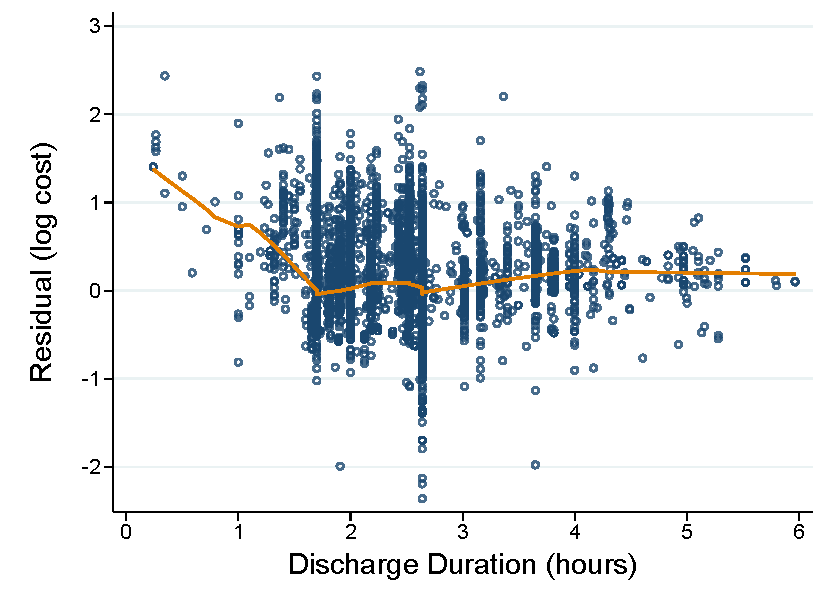
\includegraphics[width=0.5\textwidth]{CA_SGIP/cobb_douglas_resids.png}}}
	\subfloat[\centering Translog.]{{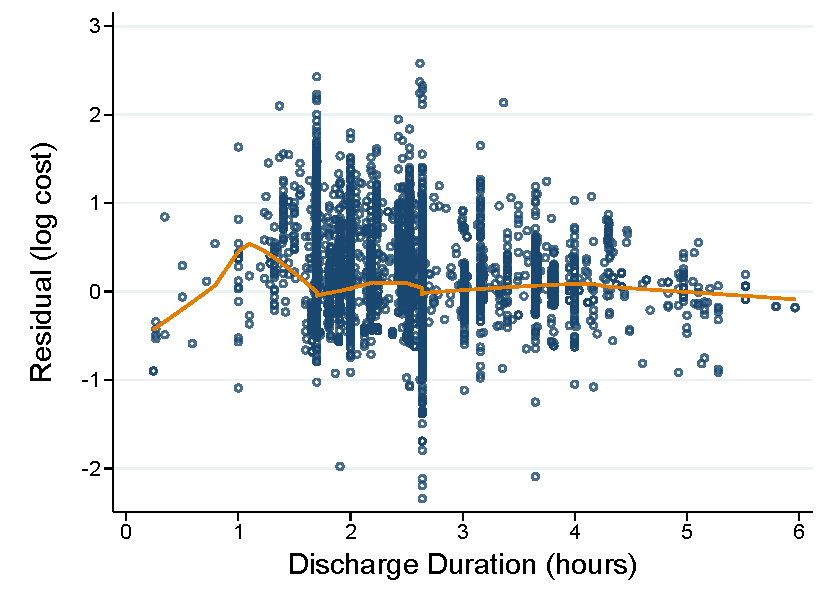
\includegraphics[width=0.5\textwidth]{CA_SGIP/translog_resids.png}}}
\caption{Comparison of Residuals from Estimation of Cobb-Douglas and Translog Models on SGIP Sample.}\label{fig:CD_vs_TL_resids}
\end{figure}

This result is likely related to the fact that 96.3\% of observations in the SGIP sample have discharge durations falling between 1.699 (corresponding to the LG RESU10, 17.1\% of the sample) and 2.64 hours (corresponding to the Tesla Powerwall 2, 62.4\% of the sample), inclusive.\footnote{SGIP reports the name of the battery manufacturer, but not the name of the battery model, which I have inferred. The discharge durations are computed from the SGIP data. SGIP requires project developers to report the energy capacity in terms of ``usable AC energy,'' so these values will not conform to calculations performed with nominal DC or usable DC values reported by the manufacturers.} Hence, the estimated parameters of both models are tightly calibrated to generate unbiased predictions within this range, whereas the residuals outside it are more liable to deviate from an expected value of zero.

A related fact is that there is extremely strong collinearity of energy and power in the SGIP data: the coefficient of correlation is 0.946. Hence, there is limited statistical leverage by which to reliably estimate the independent marginal effect of energy and power, especially outside of the narrow range of commonly observed discharge durations. This clouds the model selection decision because the two models generate very different predictions regarding marginal cost. Whereas the estimated parameters of a Cobb-Douglas model translate to a diminishing marginal cost of energy capacity, the estimated parameters of the translog model translate to an increasing marginal cost of energy capacity. I adjudicate between these competing predictions in the next section.

\subsection{Marginal Cost of Energy Capacity: Cobb-Douglas vs. Translog}\label{apdx:mc}

I investigate the possibility of overfitting by evaluating the extent to which the translog function extrapolates poorly outside the range of the most common discharge durations (1.699 to 2.64 hours). The parameters $\gamma_1$, $\gamma_2,$ and $\gamma_3$ enable curvature in the surface of best fit in the Cartesian space defined by $(\ln(E), \ln(P), \ln(C))$; curvature which marginally improves model fit for ratios of energy to power within the range of the most common values could easily be invalid outside that range. To test this hypothesis, I estimate several Cobb-Douglas models---flat surfaces of best fit in $(\ln(E), \ln(P), \ln(C))$---within restricted sample domains of discharge duration and compare the resulting estimates of marginal cost. 

It is possible that there exist omitted variables correlated with the discharge duration. In particular, manufacturers may differ in their pricing for reasons unrelated to discharge duration, yet pricing and discharge duration may be correlated. I test this hypothesis in two ways: first, I re-estimate Eq. \ref{eq:TL} with an additional set of fixed effects by manufacturer. Second, I restrict the sample domains and then test the sensitivity of the results to inclusion or exclusion of the two most common discharge durations (1.699 and 2.64 hours). These discharge durations are closely associated with the two most dominant manufacturers (LG and Tesla, respectively) in the sample.

In Table \ref{tab:MC_estimates}, I present estimates of the marginal cost of energy capacity for a 5 kW residential BESS under different model specifications. Several conclusions emerge. The first is that Eq. \ref{eq:CD} model does not generate valid predictions of marginal cost (which are presented in row 3) across the full sample domain of discharge durations. All other models agree that there are an increasing marginal costs of energy capacity. The Cobb-Douglas functional form requires that marginal cost of a variable must diminish so long as the exponent on that variable is less than one. This finding improves confidence that the translog model is appropriate---there is indeed curvature in the surface of best fit in $(\ln(E), \ln(P), \ln(C))$.

Regarding the matter of negative marginal costs found in the baseline translog model, that result nearly vanishes when manufacturer fixed effects are included. If we examine the two Cobb-Douglas models restricted to low discharge durations, we see that the negative marginal costs disappear when LG RESU 10s (1.699 hours) are excluded from the sample domain. This implies that the LG RESU 10 has lower costs than systems with shorter discharge durations for reasons unrelated to the extra energy capacity. This may reflect LG's well-established supply chain and economies of scale in the volume of batteries it manufactures. 

When considering the higher range of discharge durations, introducing manufacturer fixed effects to the translog model does not eliminate the finding of increasing marginal costs; if anything, the slope is steeper. If we limit the restrict the sample to the longer durations and estimate a Cobb-Douglas model,  exclusion of the Tesla Powerwall 2 (and any other BESS with the same discharge duration) does reduce the steepness of the marginal cost curve. This implies that the Tesla Powerwall 2 is cheaper than would be predicted on the basis of it discharge duration; given its over-representation in the sample, it distorts the shape of the marginal cost curve.

Given these conclusions, it may seem logical to add manufacturer fixed effects to the model. However, I reject this approach on the grounds that there is good reason to expect that the relative costs of competing manufacturers are liable to change over time in unpredictable ways. A firm could discover a new innovation or scale up the volume of its manufacturing; supply chain issues could increase the costs of some firms more than others; a new firm could enter the market for which no fixed effect has been estimated. As can be plainly seen in Figure \ref{fig:TSLA_cost_adv}, Tesla's cost advantage relative to its competitors has waxed and waned over time. Therefore, I reject the inclusion of manufacturer fixed effects in Eq. \ref{eq:predict_TL}.

The sensitivity of the marginal cost estimates to model specification underscores the need for more project-level data on BTM BESS with greater dispersion in the ratio of energy to power. Given the data currently available for this study, the present estimates of the marginal cost of energy capacity have uncertain validity for BTM BESS with discharge durations outside the range [1.699, 2.64] hours. Considering the balance of the evidence, I argue that the translog model best fits the currently available data.

\begin{landscape}
\begin{table}[h]
\centering
\begin{tabular}{ccc|cccccc}
\hline
\multirow{2}{*}{Model}    & \multirow{2}{*}{\begin{tabular}[c]{@{}c@{}}Sample Domain\\ (hours)\end{tabular}}     & \multirow{2}{*}{N} & \multicolumn{6}{c}{Discharge Duration (hours)} \\\cline{4-9}
                               &                                     &                                       & 1    & 2    & 3  & 4    & 5    & 6   \\ \hline
Translog (Baseline)            & {[}0, 6{]}                    & 26,154                                     & -\$344   & \$692    & \$1,135    & \$1,578    & \$2,089    & \$2,689   \\
Translog (Mfr. F.E.s) & {[}0, 6{]}                    & 26,154                                     & -\$69    & \$915    & \$1,396    & \$1,883    & \$2,433    & \$3,065   \\
Cobb-Douglas                   & {[}0, 6{]}                    & 26,154                                     & \$971    & \$755    & \$652    & \$587    & \$541    & \$507   \\
Cobb-Douglas                   & {[}0, 1.699{]}                & 6,237                                     & -\$1,320    &      &      &      &      &     \\
Cobb-Douglas                   & {[}0, 1.699)                  & 178                                     & \$448    &      &      &      &      &     \\
Cobb-Douglas                   & {[}2.64, 6{]}                 & 16,718                                     &      &      & \$1,815    & \$2,164    & \$2,480    & \$2,773   \\
Cobb-Douglas                   & (2.64, 6{]}                   & 678                                     &      &      & \$1,263    & \$1,272    & \$1,279    & \$1,285 \\ \hline  
\end{tabular}
\caption{Estimates of the marginal cost of energy capacity for a 5 kW Residential BESS under various models and restrictions of the domain of discharge duration.}\label{tab:MC_estimates}
\end{table}
\end{landscape}

\subsection{Evidence for Translog from Analogous Industries}\label{apdx:analog_AIC}

I present evidence from two industries analogous to BTM BESS to strengthen my claim that the translog functional form is a good approximation of the relationship between system size and cost for BTM BESS. In this subsection, I mirror the procedures for model comparison and selection described in \ref{apdx:model_selection}, so I restrict the discussion to only those aspects where the procedures differ.

The first industry is BTM solar PV, which is highly analogous to BTM BESS in that both industries entail labor by electricians, manufactured modules full of power electronics, and site-specific conditions that can influence installation costs. I draw on data from the TTS dataset, excluding those observations with BESS co-installed. I include two continuous variables of system size: the DC power rating of the solar array and the AC power rating of the inverter. Given the exceptionally large sample size, the model can tolerate fixed effects by month---rather than year--- without risk of overfitting. I also include fixed effects by state, to account for the differing maturity of the rooftop solar industry in different states.

Table \ref{tab:TTS_AIC} displays the Akaike information criteria (AIC) for sixteen model specifications. Translog and Cobb-Douglas perform relatively well, but the best-fitting models are those which take the cost per kilowatt of PV as the dependent variable. When examining AIC to more significant digits, the translog model outperforms the Cobb-Douglas model. Models of untransformed total cost perform the worst.

\begin{table}[t]
\centering
\begin{tabular}{|c|cccc|}\hline
Independent & \multicolumn{4}{c|}{Dependent Variable}  \\ \cline{2-5}
Variables &  \$  \Tstrut  &  \$/kW\textsuperscript{PV}  & ln(\$) & ln(\$/kW\textsuperscript{PV})  \\\hline
level, linear     &   $3.28 \times 10^7 $    &  $2.661 \times 10^7$  & $2.85 \times 10^7$  &   $2.73 \times 10^7$  \\
level, quadratic     &   $3.26 \times 10^7 $    &  $2.660 \times 10^7$  & $2.84 \times 10^7$  &   $2.73 \times 10^7$  \\
log, linear   &   $3.46 \times 10^7 $  &    $2.655 \times 10^7$  & $2.73 \times 10^7$ & $2.73 \times 10^7$   \\
log, quadratic  & $3.36 \times 10^7 $  &    $2.655 \times 10^7$  & $2.73 \times 10^7$ & $2.73 \times 10^7$   \\\hline
\end{tabular}
\caption{Akaike Information Criteria of Sixteen Models of Installed Cost of BTM Solar PV.}\label{tab:TTS_AIC}
\end{table}

The second industry I consider is large portable batteries for consumers. It is also highly analogous to BTM BESS with respect to the fact that they employ the same underlying technology, Li-ion batteries.\footnote{4\% of the sample in the portable battery survey consists of lead-acid batteries.} The two industries differ chiefly in that portable batteries require no installation labor. Table \ref{tab:portable_AIC} displays the AIC for sixteen model specifications of the relationship between manufacturer's original retail price, power capacity, and energy capacity. The comparison indicates that the translog model minimizes the information loss. These findings strengthen confidence in the appropriateness of a translog functional form for the installed cost of BTM BESS.

\begin{table}[t]
\centering
\begin{tabular}{|c|cccc|}\hline
Independent & \multicolumn{4}{c|}{Dependent Variable}  \\ \cline{2-5}
Variables &  \$ \Tstrut   &  \$/Wh  & ln(\$) & ln(\$/Wh)  \\\hline
level, linear     &   997    &  1,858 & 954  &   881  \\
level, quadratic    &   997    &  1,858 & 897  &   879  \\
log, linear    &   1,072 &    1,852  & 875 & 875   \\
log, quadratic    &   996    &  1,839 & 865  &  865  \\\hline
\end{tabular}
\caption{Akaike Information Criteria of Sixteen Models of Installed Cost of Large Portable Batteries.}\label{tab:portable_AIC}
\end{table}

\subsection{A Linear Model with Time-Varying Coefficients}\label{apdx:time_var_coef}

As noted in Subsection \ref{sec:linear_lit}, a linear model of installed cost, energy capacity, and power capacity has widrespread use in prior literture. The results in Table \ref{tab:SGIP_AIC} indicate that a simple linear model exhibits very poor fit to the data. However, the poor fit may reflect the fact that per unit costs of energy and power have been declining over time. To give full consideration to the possibilty of a linear relationship, I estimate a functional form equivalent to that of \citet{augustineblair2021} on the SGIP data: 

\begin{equation}\label{eq:augustineblair2021}
    C_i = \alpha^{s}_{t} + \beta_{1t} E_i + \beta_{2t} P_i + \varepsilon_i
\end{equation}

The parameters $\beta_{1t}$ and $\beta_{2t}$ are subscripted by year to capture falling specific costs of energy and power capacity, which \citeauthor{augustineblair2021} argue trend downward at different rates. While Eq. \ref{eq:augustineblair2021} is intuitively appealing, it fits the SGIP data poorly. When estimated on the training sample the AIC is $7.10 \times 10^5 $, which is only marginally better than a linear model in which $\beta_{1}$ and $\beta_{2}$ are constrained to be equal across all years (row 1, column 1 of Table \ref{tab:SGIP_AIC}). The relative likelihood of the \citet{augustineblair2021} model compared to the translog model---i.e., the probability that the former reduces information loss compared to the latter---is infinitesimally close to 0\%.\footnote{$\exp((7.10 \times 10^5 - 5.71 \times 10^5)/2) \approx 0\% $} Furthermore, the estimated values of $\alpha^{s}_{t}$, $\beta_{1t}$, and $\beta_{2t}$ vary wildly across years, as is presented in Figures \ref{fig:linear_fc}, \ref{fig:linear_ecc}, and \ref{fig:linear_pcc}, rather than following a steady pattern of cost decline or exhibiting modest increases in recent years. In some years the point estimates are negative; in others, they are far larger than is credible. This strongly suggests that allowing $\beta_{1}$ and $\beta_{2}$ to vary by year results in overfitting of the model.

\begin{figure}[b!]
\centering
\includegraphics[width=\textwidth]{CA_SGIP/linear_fc.pdf}
\caption{Estimated value of $\alpha^{R}_{t}$ from Eq. \ref{eq:augustineblair2021} by year.}\label{fig:linear_fc}
\end{figure}

\begin{figure}[p]
\centering
\includegraphics[width=0.9\textwidth]{CA_SGIP/linear_ecc.pdf}
\caption{Estimated value of $\beta_{1t}$ from Eq. \ref{eq:augustineblair2021} by year.}\label{fig:linear_ecc}

\includegraphics[width=0.9\textwidth]{CA_SGIP/linear_pcc.pdf}
\caption{Estimated value of $\beta_{2t}$ from Eq. \ref{eq:augustineblair2021} by year.}\label{fig:linear_pcc}
\end{figure}

\newpage

\section{Estimation Results of the Cobb-Douglas Model}\label{apdx:cobb_douglas}

Table \ref{reg:predict_CD} presents the estimated parameters of Eq. \ref{eq:predict_CD}, the Cobb-Douglas equivalent to Eq. \ref{eq:predict_TL}. In this appendix, I discuss the interpretation of the results.

\begin{align}
    \ln(C_i) = &~\alpha^{s}_{t} + \beta_1 \ln(E_i) + \beta_2 \ln(P_i) + \delta_1 AC_i + \delta_2 DC_i  \label{eq:predict_CD} \\
		 & + \delta_3 ln(w^{c}_{t}) + \varepsilon_i \nonumber
\end{align}

\begin{table}[t]
\centering
\begin{tabular}{lcc} \hline
\Tstrut                       & \multicolumn{2}{c}{\textbf{Scale Parameters}}                    \\ \cline{2-3} 
\Tstrut   \Bstrut                    & \textit{Energy} ($\beta_1$)             & \textit{Power} ($\beta_2$)              \\
                      & 0.637 (0.030)                    & 0.217 (0.031)                     \\
[0.5em]
  & \multicolumn{2}{c}{\textbf{Coupling with DG}}                    \\ \cline{2-3} 
\Tstrut   \Bstrut & \textit{AC} ($\delta_1$) & \textit{DC} ($\delta_2$) \\
                      & 0.025 (0.018)                    & 0.003 (0.022)                     \\
[0.5em]
\Bstrut                    & \multicolumn{2}{c}{\textit{Hourly Wage of Electricians} ($\delta_3$)}                    \\
                      & \multicolumn{2}{c}{0.023 (0.008) }                                       \\
[0.5em]
                      & \multicolumn{2}{c}{\textbf{Sector-Year Fixed Effects} ($\alpha^s_t$)} \\ \cline{2-3} 
\textit{year}	\Tstrut \Bstrut  & \textit{Residential}                   & \textit{Non-Residential}            \\
2013                  &   8.49 (0.04)                         &        8.41 (0.10)                    \\
2014                  &   8.17 (0.04)                         &        8.40 (0.06)                    \\
2015                  &   8.20 (0.04)                         &        8.27 (0.05)                    \\
2016                  &   8.17 (0.06)                         &        8.32 (0.06)                    \\
2017                  &   7.08 (0.05)                         &        8.01 (0.06)                    \\
2018                  &   7.16 (0.05)                         &        7.93 (0.05)                    \\
2019                  &   7.28 (0.05)                         &        7.82 (0.05)                    \\
2020                  &   7.42 (0.05)                         &        7.77 (0.06)                    \\
2021                  &   7.48 (0.05)                         &        7.68 (0.06)                    \\ \cline{1-3} 
\multicolumn{3}{r}{\footnotesize \tstrut N = 28,532  \quad   adj. R\textsuperscript{2}=0.884   \quad  RMSE = 0.267}     \\  \cline{1-3}            
\multicolumn{3}{l}{\footnotesize \textit{Robust standard errors in parentheses.}}           
\end{tabular}
\caption{Estimated Parameters of Eq. \ref{eq:predict_CD}}\label{reg:predict_CD}
\end{table}

\subsection{Scale Parameters}\label{apdx:scale_CD}

The scale parameter for energy capacity ($\beta_1$) is estimated to be 0.637 ($\pm$ 0.060) and the scale parameter for power capacity ($\beta_2$) is estimated to be 0.217 ($\pm$ 0.061). The sum of these two parameters is 0.854 ($\pm$ 0.009), which indicates that BTM BESS exhibits moderate economies of scale. The interpretation of this number is that simultaneously increasing the energy capacity and power capacity by an order of magnitude is predicted to reduce the average cost per kilowatt-hour by approximately 28.6\% ($\pm$ 1.5\%).\footnote{$10^{0.854-1}-1=-0.286$}

As indicated by the margins of error in parentheses, there is greater uncertainty in the estimates of the individual parameters than their sum. This is a consequence of the high collinearity of energy and power capacity. It is unfortunate that nearly all of the variation in the ratio of energy to power in the SGIP sample arises primarily from the moderately different product sizing decisions of the two most dominant manufacturers in the market, Tesla and LG. This means that estimates of the marginal effect of energy or power, while holding the other constant, are not credibly disentangled from any potentially important but unobserved differences in the design of the BESS that is associated with the identity of the manufacturer.

For example, Tesla requires the installation of its proprietary ``Backup Gateway,'' an internet-connected device that monitors and controls the behavior of the Powerwall, solar inverters, solar panels, and the customer's grid connection. In comparison, LG instructs its customers to buy an inverter that pairs with the RESU10 and performs similar functions. The RESU10 is a DC-coupled battery, so the cost of the inverter is inframarginal for the typical consumer planning to go solar and deciding whether to add a BESS or not. Since the RESU10 and Powerwall 2 have identical power capacity but the energy capacity of the Powerwall 2 is larger, ordinary least squares may wrongly infer that the additional costs arising from Tesla's Backup Gateway are a type of cost that scales with a higher ratio of energy to power. In reality, the Backup Gateway is a fixed cost: Tesla customers need only purchase one Backup Gateway, which can manage up to ten Powerwalls.

To evaluate the sensitivity of the scale parameters to this issue, I augment Eq. \ref{eq:predict_CD} with an additional fixed effect corresponding to the identity of the battery manufacturer. Estimating this modified regression on the SGIP data returns $\hat{\beta}_1 = 0.781$ ($\pm$ 0.071) and $\hat{\beta}_2 = 0.119$ ($\pm$ 0.070). The sum of these parameters is 0.901 ($\pm$ 0.008). Again, the degree of economies of scale can be pinned down with a high degree of confidence, whereas the individual parameters for the marginal effects of power and energy are more uncertain.

For a point of comparison, I estimate a Cobb-Douglas model of large portable batteries, with an assortment of fixed effects.\footnote{There are no sector fixed effects as these products are marketed predominantly to household consumers. There are no year fixed effects, since all the data were gathered within a single narrow window of time.} The results are presented in Table \ref{reg:CD_portable}. The scale parameters vary slightly from specification to specification, but broadly they are in agreement that a much greater weight---between 4 and 6 times greater---on the energy capacity relative to the power capacity. Unlike stationary BTM BESS, large portable batteries do not exhibit statistically significant economies of scale (formally, we cannot reject the hypothesis that $\beta_1 + \beta_2 \geq 1$).

\begin{table}[t]
\centering
\newcolumntype{Y}{>{\centering\arraybackslash}X}

\begin{tabularx}{0.8\textwidth}{lYYY}
\hline\hline
            &\multicolumn{1}{c}{(1)}&\multicolumn{1}{c}{(2)}&\multicolumn{1}{c}{(3)}\\
\hline
Energy Capacity       &       0.792&       0.839&       0.758 \Tstrut\\
\textit{ln(Wh)}            &      (0.055)&      (0.053)&      (0.064)\\
[0.5em]
Power Capacity     &       0.165&       0.137&       0.195\\
\textit{ln(W)}            &      (0.054)&      (0.053)&      (0.055) \Bstrut \\ \hline
Fixed Effects & None & Chemistry & Manufacturer \\
Observations      &          69&          69&          68\\
\hline\hline
\multicolumn{4}{l}{\footnotesize \textit{Robust standard errors in parentheses.}}\\
\end{tabularx}
\caption{Cobb-Douglas Model of the Retail Price of Large Portable Batteries}\label{reg:CD_portable}
\end{table}

\subsection{Sector-Year Fixed Effects}\label{apdx:CD_trends}

\begin{figure}[t]
\includegraphics[width=\textwidth]{graphs/CA_SGIP/CSCI_CD.pdf}
\caption{Sector-Year Fixed Effects from Eq. \ref{eq:CD}, normalized such that $\alpha^{Res.}_{2016} = 100$}\label{fig:CSCI_CD}
\end{figure}

Figure \ref{fig:CSCI_CD} presents the estimated sector-year fixed effects of Table \ref{reg:predict_CD} in a visual format. For ease of interpretation, I have normalized all values such that the fixed effect for the residential sector in 2016 is equal to 100, following Eq. \ref{eq:CSCI}. The sector-specific trends estimated by the Cobb-Douglas model are virtually indistinguishable from those estimated by the translog model (\textit{cf.} Figure \ref{fig:CSCI_TL}).

\section{Derivation of the Interpretation of the Parameters of the Translog Cost Function for BTM BESS}\label{apdx:TL_interpretation}

This appendix presents the derivation of the interpretation of the parameters of the translog cost function (Eq. \ref{eq:predict_TL}), which I present again below for the convenience of the reader:

\begin{align*}
    \ln(C_i) = &~\alpha^{s}_{t} + \beta_1 \ln(E_i) + \beta_2 \ln(P_i) + \gamma_1 \ln(E_i)^2 + \gamma_2 \ln(P_i)^2  \tag{\ref{eq:predict_TL}} \\
		 & + \gamma_3 \ln(E_i) \ln(P_i) + \delta_1 AC_i + \delta_2 DC_i + \delta_3 \ln(w^{c}_{t}) + \varepsilon_i \nonumber
\end{align*}

Throughout this appendix, I omit the subscript $i$ (denoting individual observations) to streamline the presentation. 

\subsection{Marginal Costs of Energy Capacity, Power Capacity and Discharge Duration}\label{apdx:mc_derivation}

In this section, I derive the marginal costs of extending the energy capacity ($MC_{E}$) and power capacity ($MC_{P}$). I also derive the related marginal cost of extending the discharge duration ($MC_{D}$), which is slightly different way of expressing the marginal cost of extending energy capacity.

\begin{subequations}\label{eq:MC_defs}
\begin{align}
	MC_{E} \equiv &~\frac{\partial C}{\partial E}\Big\rvert_{P} \label{eq:MCe_def} \\
	MC_{P} \equiv &~\frac{\partial C}{\partial P}\Big\rvert_{E}\label{eq:MCp_def} \\
	MC_{D} \equiv &~\frac{\partial C}{\partial D}\Big\rvert_{P}  \label{eq:MCd_def} 
\end{align}
\end{subequations}

The partial derivative of the natural log of installed cost with respect to any of the variables of interest ($X$, for generality) exhibits a useful relationship to Eq. \ref{eq:predict_TL} and the marginal costs defined in Eqs. \ref{eq:MC_defs}:

\begin{align}\label{eq:MC_TC}
	\frac{\partial \ln(C)}{\partial X} = \frac{\frac{\partial C}{\partial X}}{C} = \frac{MC_X}{C} \notag \\
	MC_X = C \cdot \frac{\partial \ln(C)}{\partial X}
\end{align}

In words, ``the marginal cost is equal to the installed cost times the percentage change of installed cost arising from a incremental change in $X$.'' This step eliminates the need to exponentiate Eq. \ref{eq:predict_TL} before computing its partial derivatives:

\begin{subequations}\label{eq:lnTC_partials}
\begin{align}
    \frac{\partial \ln(C)}{\partial E} &= \frac{\beta_1 + 2 \gamma_1 \ln(E) + \gamma_3 \ln(P)}{E} \label{eq:lnTC_partial_e} \\
    \frac{\partial \ln(C)}{\partial P} &= \frac{\beta_2 + 2 \gamma_2 \ln(P) + \gamma_3 \ln(E)}{P} \label{eq:lnTC_partial_p} \\
    \frac{\partial \ln(C)}{\partial D} &= \frac{\beta_1 + 2 \gamma_1[\ln(P)+\ln(D)] + \gamma_3 \ln(P)}{D} \label{eq:lnTC_partial_d}
\end{align}
\end{subequations}

However, Eq. \ref{eq:predict_TL} must be reverse log-transformed before it can be substituted into Eq. \ref{eq:MC_TC}. This is a fairly trivial matter, except for the issue of the error term. While  $\varepsilon$ is zero in expectation, $\exp(\varepsilon)$ is not. The standard correction for retransformation bias of any model with a log-transformed dependent variable is to substitute one-half the square of the root-mean-square error (RMSE) in place of the error term before exponentiation \citep{miller1984}. Thus, the predicted value of installed cost ($\widehat{C}$) is given by:

\begin{equation}\label{eq:TC_hat}
\begin{split}
\widehat{C} =  & E^{\beta_1} P^{\beta_2} \exp(\alpha^{s}_{t} + \gamma_1 \ln(E)^2 + \gamma_2 \ln(P)^2 \\
		 & + \delta_1 AC_i + \delta_2 DC_i + \delta_3 \ln(w^{c}_{t}) + 0.5 RMSE^2)
\end{split}
\end{equation}

Finally, I substitute Eq. \ref{eq:TC_hat} and Eqs. \ref{eq:lnTC_partials} into Eq. \ref{eq:MC_TC} to produce the final result. 

\begin{subequations}\label{eq:MC_results}
\begin{align}
    MC_{E} =&~[\beta_1 + 2 \gamma_1 \ln(E) + \gamma_3 \ln(P)] E^{\beta_1-1} P^{\beta_2}  \label{eq:MCe_result} \\ & exp(\alpha^{s}_{t} + \gamma_1 \ln(E)^2 + \gamma_2 \ln(P)^2 \notag \\
    & + \gamma_3 \ln(E) \ln(P) + 0.5 RMSE^2) \notag \\
    MC_{P} =&~[\beta_2 + 2 \gamma_2 \ln(P) + \gamma_3 \ln(E)] E^{\beta_1} P^{\beta_2-1}  \label{eq:MCp_result} \\ & exp(\alpha^{s}_{t} + \gamma_1 \ln(E)^2 + \gamma_2 \ln(P)^2 \notag \\
    & + \gamma_3 \ln(E) \ln(P) + 0.5 RMSE^2) \notag \\
    MC_{D}  =&~[\beta_1 + 2 [\gamma_1 \ln(P) + \ln(D)] + \gamma_3 \ln(P)] D^{\beta_1-1} P^{\beta_1+\beta_2}  \label{eq:MCd_result} \\ & exp(\alpha^{s}_{t} + \gamma_1 [\ln(P)+\ln(D)]^2 + \gamma_2 \ln(P)^2 \notag \\
    & + \gamma_3 [\ln(P)+\ln(D)] \ln(P) + 0.5 RMSE^2) \notag 
\end{align}
\end{subequations}

Observe that in Eqs. \ref{eq:lnTC_partial_d} and \ref{eq:MCd_result}, I decompose $E$ into $P$ and $D$. This clarifies that, in computing $MC_D$, the power rating is held constant while sufficient energy capacity is added to extend the discharge duration. With $MC_E$, the interpretation is that exactly one kilowatt-hour of energy capacity is to be added; the extent to which such an addition extends discharge duration will vary with the power rating of the BESS.

\subsection{Economies of Scale}\label{apdx:eos_derivation}

The degree of economies (or diseconomies) of scale intrinsic to the installed cost of a BTM BESS is characterized by:

\begin{equation}\label{eq:eos_def}
    \eta \equiv \frac{C(\theta E, \theta P)}{\theta C(E, P)}
\end{equation}

$\theta$ represents any arbitrary increase (if greater than one) or decrease (if less than one) in the size of the system realtive to some baseline size ($E, P$). $\eta$ represents the ratio of the installed cost a single system sized ($\theta E$, $\theta P$) relative the installed cost of $\theta$ systems sized ($E$, $P$). For the case of $\theta >1$, the installed cost function is said to exhibit economies of scale when $\eta$ is less than one, or diseconomies of scale when $\eta$ is greater than one.

I log-transform Eq. \ref{eq:eos_def} and substitute in Eq. \ref{eq:predict_TL}:

\begin{align*}
\ln(\eta) =&~\ln(C(\theta E, \theta P))-\ln(\theta) - \ln(C(E, P)) \\
\ln(\eta) =&~[\alpha^{s}_{t} + \beta_1 \ln(\theta E) + \beta_2 \ln(\theta P) + \gamma_1 \ln(\theta E)^2 + \gamma_2 \ln(\theta P)^2 \\ 
		 & + \gamma_3 \ln(\theta E) \ln(\theta P) + ... + \varepsilon] - \ln(\theta) - [\alpha^{s}_{t} + \beta_1 \ln(\theta E) + \beta_2 \ln(\theta P) \\ 
		 & + \gamma_1 \ln(\theta E)^2 + \gamma_2 \ln(\theta P)^2 + \gamma_3 \ln(\theta E) \ln(\theta P) + ... + \varepsilon] \\ 
\ln(\eta) =&~(\beta_1 + \beta_2 -1) \ln(\theta) + \gamma_1[2 \ln(E) \ln(\theta) + \ln(\theta)^2] \\ 
        & + \gamma_2[2 \ln(P) \ln(\theta) + \ln(\theta)^2] + \gamma_3 [\ln(\theta)\ln(E) + \ln(\theta)ln(P)+\ln(\theta)^2] \\ 
\ln(\eta) =&~\big[\beta_1 + \beta_2 -1 + \gamma_1[2 \ln(E) + \ln(\theta)] + \gamma_2[2 \ln(P) + \ln(\theta)]\\
        &~+ \gamma_3 [\ln(E) + \ln(P)+ln(\theta)]\big]\ln(\theta) \\ 
\end{align*}

Finally, I undo the log-transformation\footnote{In this case, the error terms cancelled out, so retransformation bias does not enter under this operation.} to arrive at a closed-form solution for $\eta$:
\begin{equation}\label{eq:eos_TL}
\begin{split}
\eta   =\theta^{\beta_1 + \beta_2 -1 + (\gamma_1 + \gamma_2 + \gamma_3) \ln(\theta) + (2\gamma_1 + \gamma_3) \ln(E) + (2\gamma_2 + \gamma_3) \ln(P)}\\ 
\end{split}
\end{equation}

Eq. \ref{eq:eos_TL} reveals that, for the translog cost function, $\eta$ is a function not only of $\theta$ but also the baseline values of E and P against which different system sizes are compared. For comparison, the equivalent expression for a Cobb-Douglas model of installed cost is:

\begin{equation}\label{eq:eos_CD}
\eta   =\theta^{\beta_1 + \beta_2 -1} \\ 
\end{equation}

\section{Prediction Intervals}\label{apdx:prediction_interval}

As discussed in Subsection \ref{sec:lit_uncertainty}, there is a difference between uncertainty in the mean and uncertainty attributable to variance in individual outcomes. A common convention is to distinguish between these two types of uncertainty by reserving the term ``confidence interval'' for bounding uncertainty in the mean (such as of parameter or the condition mean of the outcome) and using the term ``prediction interval'' to refer to bounds on uncertainty of an individual prediction. Both intervals are centered on the best estimate of the mean, but they differ in their standard errors.

Under the classical assumption of normally distributed errors, the standard error for uncertainty in the mean of the dependent variable conditional on a vector of independent variables $\vec{x}_0$ is given by:

\begin{equation} \label{eq:se_c}
se_{c} = RMSE \sqrt{\vec{x}_0' (X'X)^{-1} \vec{x}_0}
\end{equation}

where RMSE is the root mean squared error and $X$ is a matrix containing all the data on the independent variables. The term under the square root is decreasing in sample size and is often less than one. Thus, a value of $se_{c}$ far less than $RMSE$ is fairly typical. For comparison, the standard error for uncertainty (again, assuming normally distributed errors) in the prediction is given by:

\begin{equation} \label{eq:se_p}
se_{p} = RMSE \sqrt{1+\vec{x}_0' (X'X)^{-1} \vec{x}_0}
\end{equation}

The term in the square root is bounded from below by one. Thus, $se_{p}$ cannot be less than RMSE. In the online code appendix, I find that that sample-weighted average value of $se_{p}$ is only 0.05\% larger than the RMSE; for all practical purposes, RMSE is a sufficient measure of prediction uncertainty. Nevertheless, the online code appendix contains code by which $se_{p}$ can be calculated for any particular $\vec{x}_0$, if desired. 

The range of a 95\% prediction interval associated with a prediction generated by Eq. \ref{eq:predict_TL} can be expressed in percentage terms with some algebra. All variables and notation not previously defined are defined in Table \ref{tab:PI_notation}.

 \begin{align*}
    \ln(C_i) = &~\alpha^{s}_{t} +\beta_1 \ln(E_i) +... + \delta_3 \ln(w^{c}_{t}) + \varepsilon_i \tag{\ref{eq:predict_TL}} \\
    \ln(C_{n+1}) = &~\alpha^{s}_{t} +\beta_1 \ln(E_{n+1}) +... + \delta_3 \ln(w^{c}_{t}) + \varepsilon_{n+1} \notag \\
   (\ln(\underline{C}_{n+1}),\ln(\overline{C}_{n+1}))= &~\alpha^{s}_{t} + \beta_1 \ln(E_{n+1}) + ... + \delta_3 \ln(w^{c}_{t}) \pm z_{\alpha/2} \times RMSE \notag \\
   (\underline{C}_{n+1}, \overline{C}_{n+1}) = &~\exp(\alpha^{s}_{t} +\beta_1 \ln(E_{n+1})  ... + \delta_3 \ln(w^{c}_{t})) \exp(\pm z_{\alpha/2} \times RMSE ) \notag  \\
   PI_{n+1} = &~\widehat{C}_{n+1} \times \exp(\pm z_{\alpha/2} \times RMSE ) \tag{\ref{eq:pi_normal}} \\
\end{align*}

For $\alpha = 0.95$ and RMSE = 0.263, the term $\exp(\pm z_{\alpha/2} \times RMSE)$ equates to (0.593, 1.686). Thus, the 95\% prediction interval can be expressed as (-40.7\%, +68.8\%) of the best estimate of the installed cost.

If one uses the assumes that the errors are Laplace distributed, then one should substitute the quantiles of a Laplace distribution associated with coverage probability $\alpha$ in place of $\pm z_{\alpha/2} \times RMSE$. The Laplace distribution in question should be calibrated to match the empirical distribution of residuals, namely: the location parameter ($\widehat{\mu}$) should be set equal to the median of the residuals ($\widehat{e}_i$) and the scale parameter ($\widehat{b}$) should be set equal to the mean absolute deviation of the residuals from the median \citep{kotz2001}:

\begin{equation}
\widehat{b} = \frac{1}{n-2} \sum^{n}_{i=1}  |\widehat{e}_i - \widehat{\mu}|
\end{equation}

The lower ($\underline{Q}(\alpha)$)and upper ($\overline{Q}(\alpha)$) quantiles associated with $1 - \alpha$ coverage probability for a Laplace distribution with location parameter $\widehat{\mu}$ and scale parameter $\widehat{b}$ can be computed from the inverse cumulative distribution function of the Laplace distribution \citep{kotz2001}. The computation of these quantiles simplifies to:

\begin{equation}
(\underline{Q}(\alpha), \overline{Q}(\alpha)) = \widehat{\mu} \pm \widehat{b} \ln(\alpha)
\end{equation}

Hence, the prediction interval under the assumption of Laplace distributed errors equals:

\begin{equation}\label{eq:pi_laplace}
PI_{n+1} = \widehat{C}_{n+1} \times \exp( \widehat{\mu} \pm \widehat{b} \ln(\alpha) ) \\
\end{equation}

\begin{table}[t]
\centering
\renewcommand\tabularxcolumn[1]{m{#1}}

\begin{tabularx}{\textwidth}{c>{\hsize=1.0\hsize\linewidth=\hsize}X}
\hline
\Tstrut  Variable     & Definition                                          \\ \hline
\Tstrut   $C_{n+1}$     & the installed cost of a non-yet-observed BTM BESS \Tstrut                                  \\ \hline
\Tstrut   $\widehat{C}_{n+1}$ & the point estimate of $C_{n+1}$                                                            \\ \hline
\Tstrut  $\underline{C}_{n+1}$   & the lower bound of a prediction interval around $C_{n+1}$                            \\ \hline
\Tstrut   $\overline{C}_{n+1}$  & the upper bound of a prediction interval around $C_{n+1}$                             \\ \hline
\Tstrut   $PI_{n+1}$    & the prediction interval around $C_{n+1}$ \\ \hline
   $z_{\alpha/2}$  & \tstrut two-sided critical value associated with coverage probability $1 - \alpha$ for a standard normal distribution \\ \hline
\Tstrut  RMSE     & root mean squared error                                                             \\ \hline                                         
\end{tabularx}
\caption{Notation and variable definitions for the derivation of Eq. \ref{eq:pi_normal}}\label{tab:PI_notation}
\end{table}


\end{document}

\endinput
%%
%% End of file `elsarticle-template-harv.tex'.
